\documentclass[11pt,compress]{beamer}
% deactivate beamer navigation
%\setbeamertemplate{navigation symbols}{}
%\usepackage{geometry}
%\geometry{papersize={180mm, 135mm}, top=-1.5mm} % 210mm, 297mm
\usepackage{../../style/lmu-lecture}
\setbeamertemplate{frametitle}{\expandafter\uppercase\expandafter\insertframetitle}

\usepackage{tikz}

\usepackage{setspace}


\AtBeginSection[]
{
  \begin{frame}<beamer>
    \frametitle{Introduction to Machine Learning}
  \begin{minipage}{\textwidth}
  %decrease linespacing to display all points
  \linespread{0.01}\selectfont
  \begin{spacing}{0.001}
  \begin{small}
  \tableofcontents[currentsection, subsectionstyle=hide]
  \end{small}
  \end{spacing}
  \end{minipage}
  \end{frame}
}
% includepdf slides, pagecommad will set counter for framenumber
\usepackage{pdfpages}
\includepdfset{trim=0mm 0mm 0mm 0mm, pagecommand={\global\setcounter{framenumber}{\value{page}}}}
% trim=0mm 6mm 0mm 0mm, offset=0 15,
% add footer:
  \usepackage{framed, color}
\usepackage{xcolor}
%\iffalse
\setbeamertemplate{footline}[text line]{%
  \noindent\hspace*{\dimexpr-\oddsidemargin-1in\relax}%
  \colorbox{white}{
    \makebox[\dimexpr\paperwidth-2\fboxsep\relax]{
      \color{black}
      \begin{minipage}[c][4.5ex][c]{0.5\linewidth}
      \secname
      \end{minipage}
      \hfill\begin{minipage}[c][4.5ex][c]{0.5\linewidth}
      \flushright
      \insertframenumber{}~/~\inserttotalframenumber~~
        \end{minipage}
    }}%
  \hspace*{-\paperwidth}
}
%\fi


\title{
  \hspace{-0.5cm}\centerline{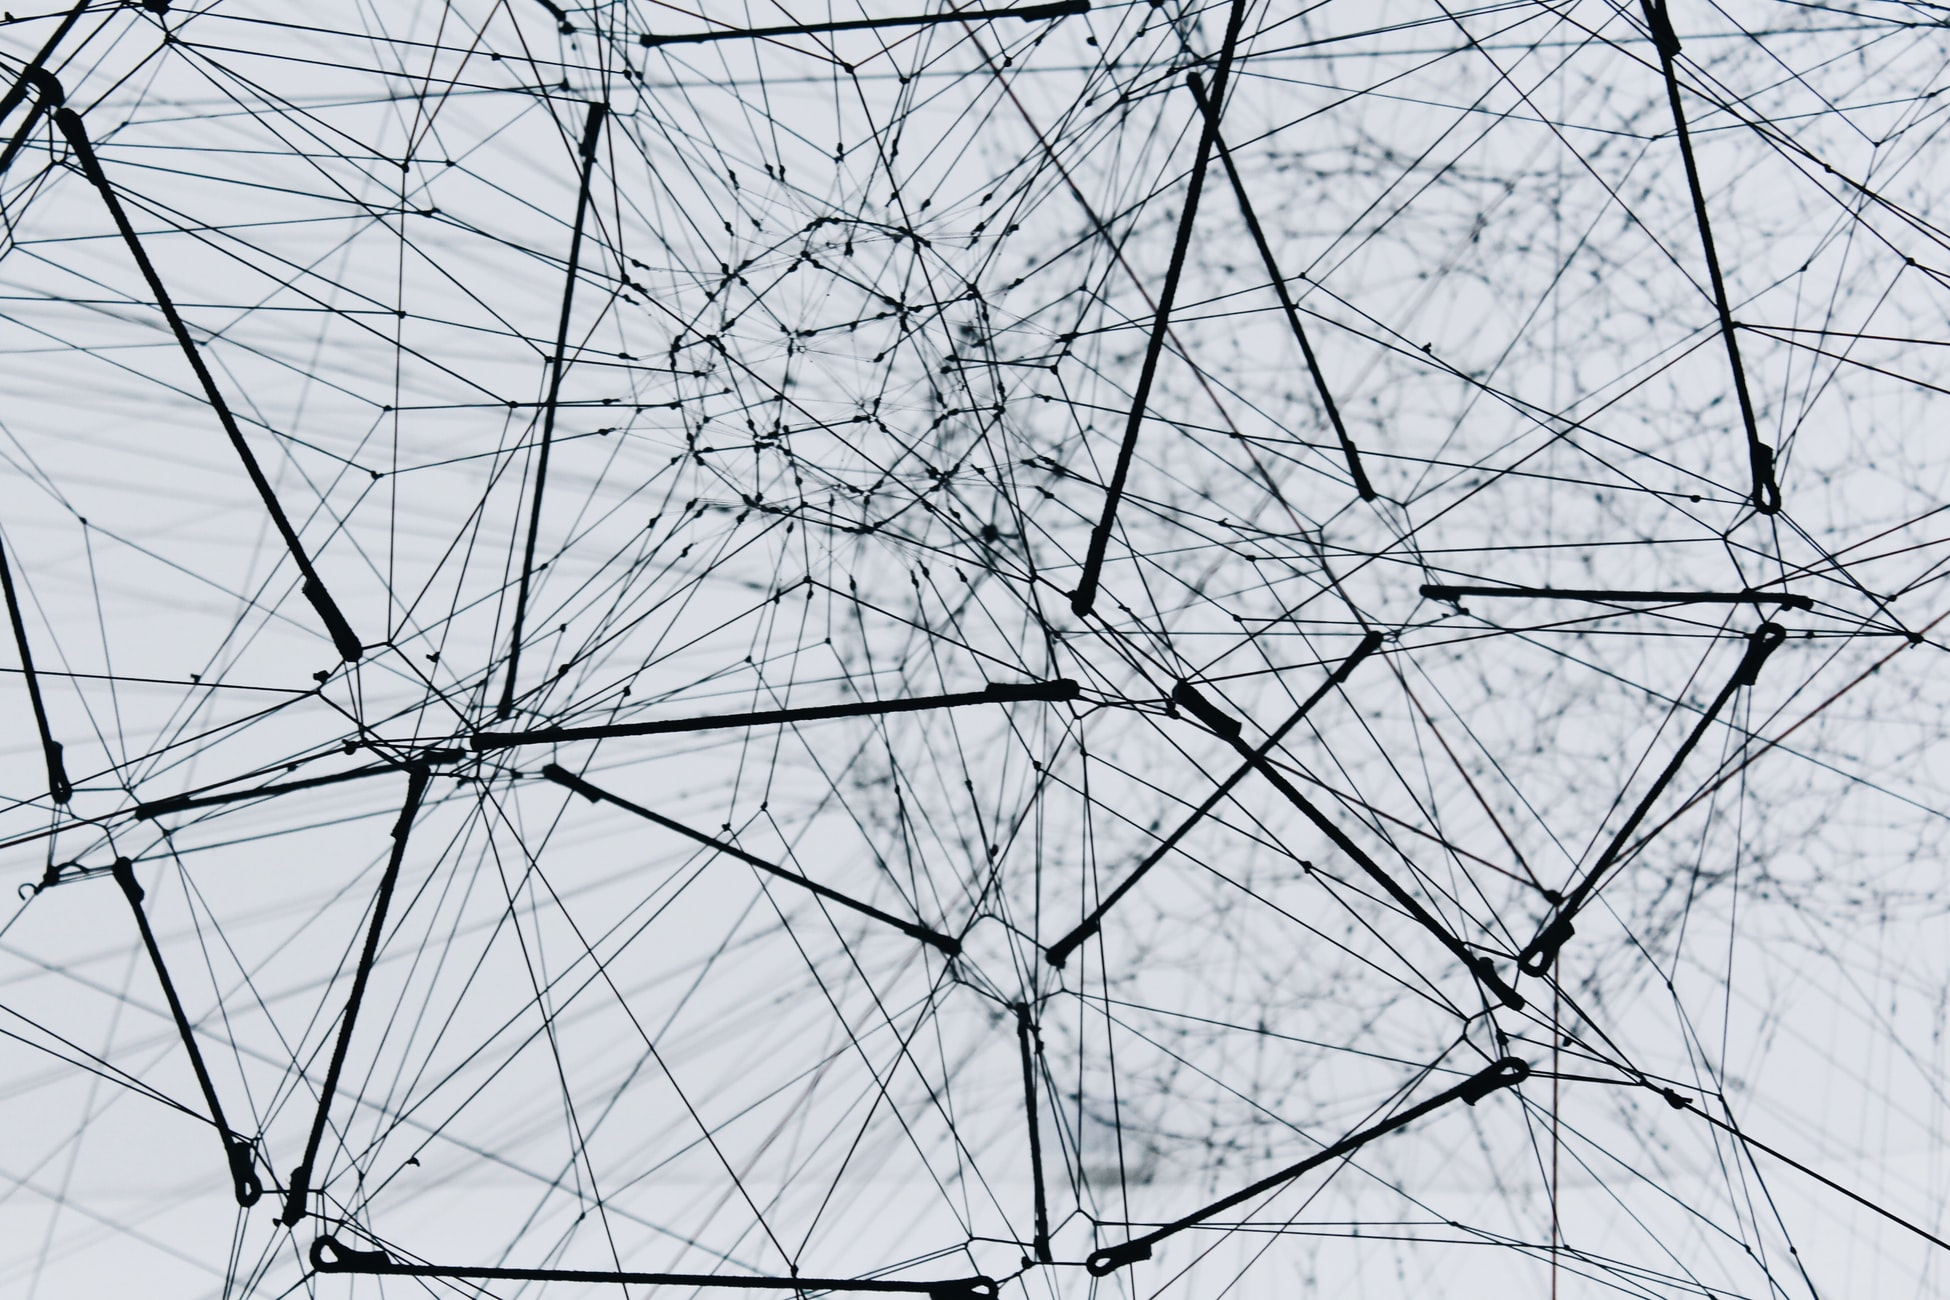
\includegraphics[width=1.05\paperwidth,keepaspectratio, trim={0 15cm 0 5cm}, clip]{titlepage.jpg}}
  \medskip
  Supervised Learning \\
  \medskip
  \small All slides
  \vspace{-1.5cm}
}



\begin{document}
\setbeamercolor{background canvas}{bg=}

\begin{frame}[noframenumbering,plain]
\maketitle
\end{frame}


% General remark: hyperlinks in included pdfs are not clickable anymore in the combined pdf

% Include tuning lecture slides
\section{Advanced Risk Minimization}
\subsection{Risk Minimization Basics}
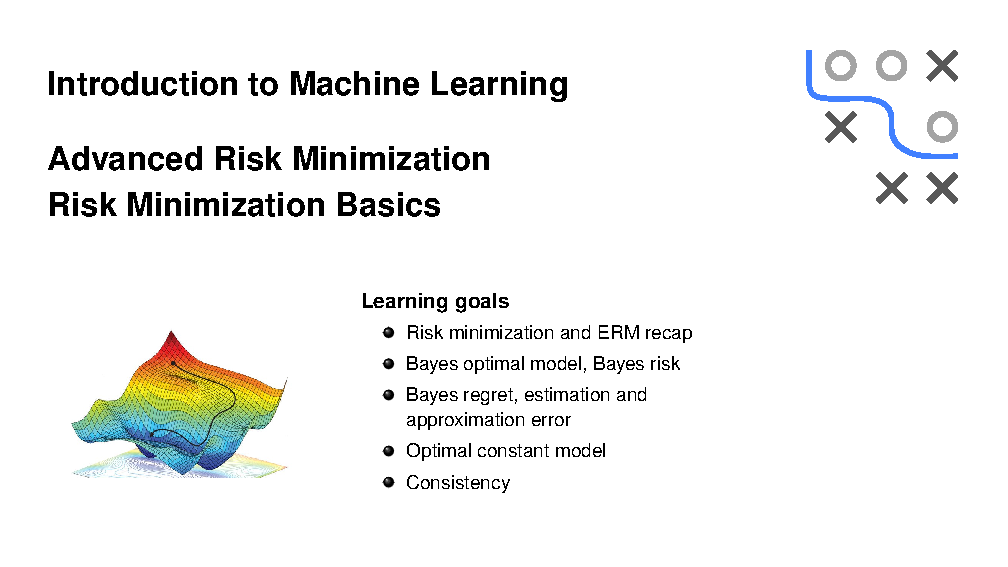
\includepdf[pages=-]{../../slides-pdf/slides-advriskmin-risk-minimization-basics.pdf}

\subsection{Loss Properties}
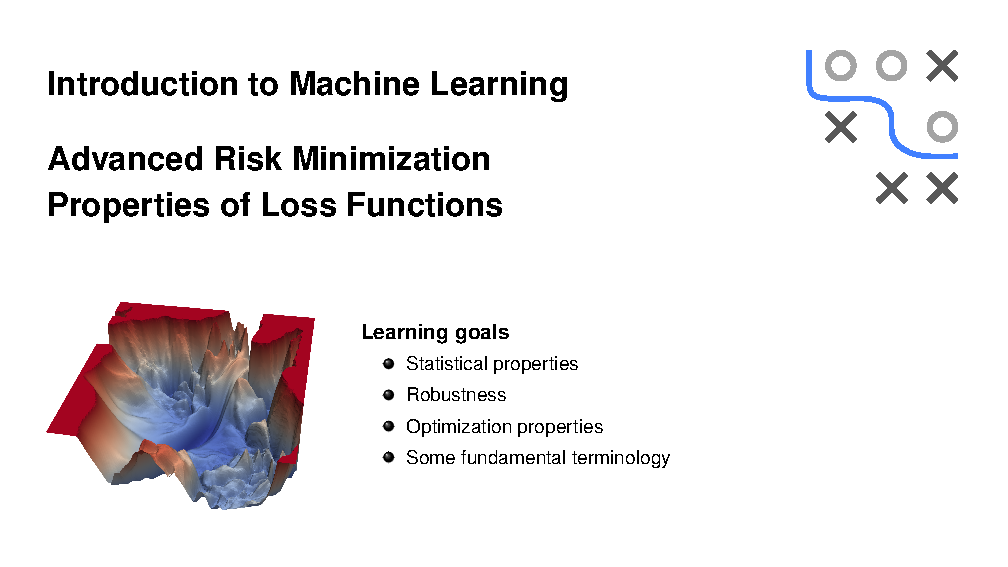
\includepdf[pages=-]{../../slides-pdf/slides-advriskmin-losses-properties.pdf}

\subsection{Pseudo-Residuals}
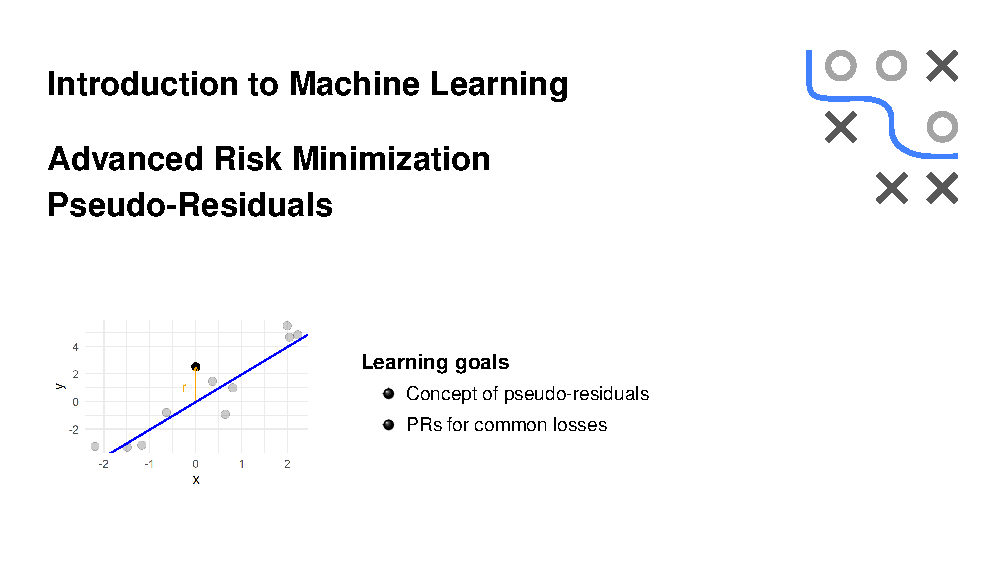
\includepdf[pages=-]{../../slides-pdf/slides-advriskmin-pseudo-residuals.pdf}

\subsection{L2- and L1-loss}
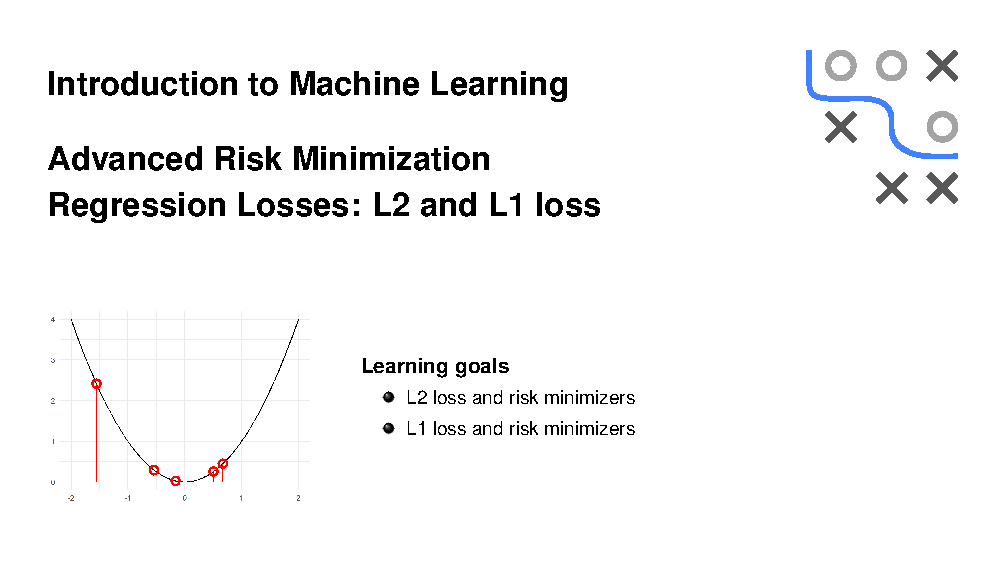
\includepdf[pages=-]{../../slides-pdf/slides-advriskmin-regression-l2-l1.pdf}

\subsection{L1 Risk Minimizer (Deep-Dive)}
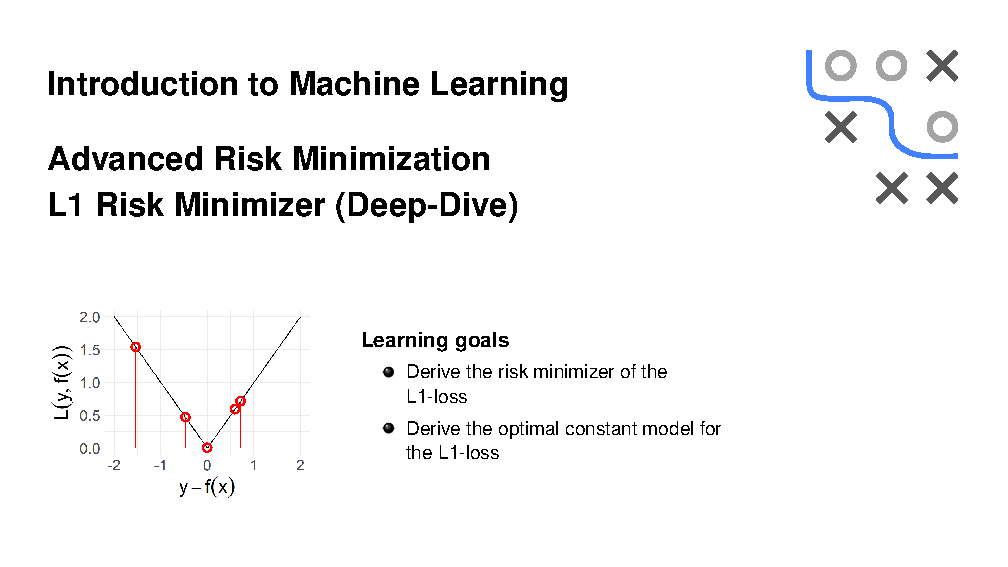
\includepdf[pages=-]{../../slides-pdf/slides-advriskmin-regression-l1-deepdive.pdf}

\subsection{Advanced Regression Losses}
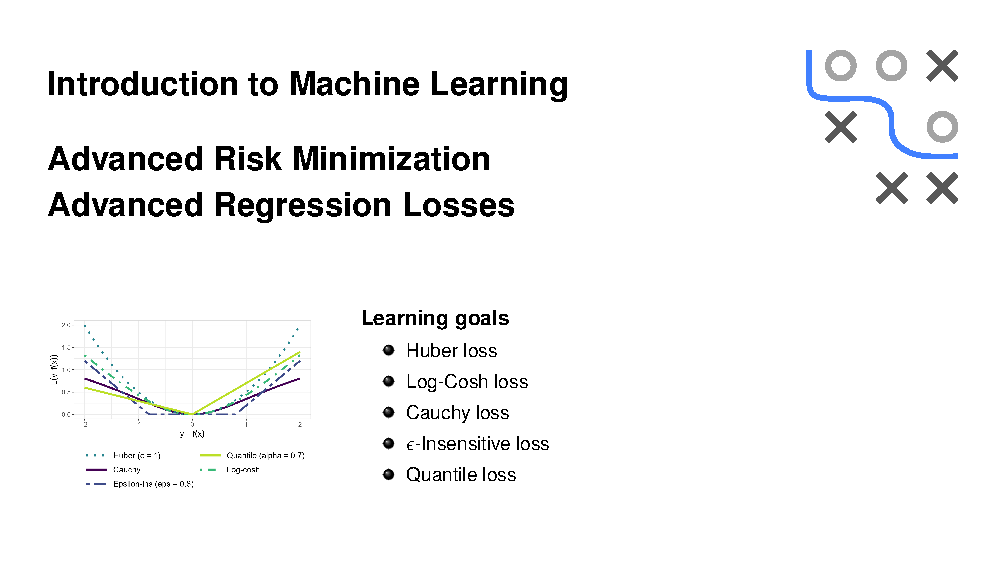
\includepdf[pages=-]{../../slides-pdf/slides-advriskmin-regression-further-losses.pdf}

\subsection{0-1-loss}
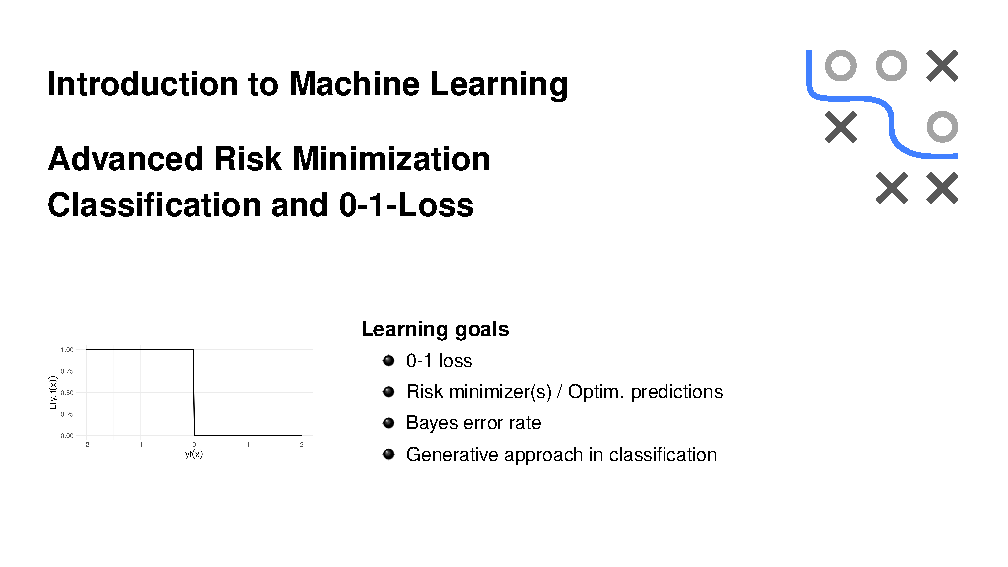
\includepdf[pages=-]{../../slides-pdf/slides-advriskmin-classification-01.pdf}

\subsection{Bernoulli Loss}
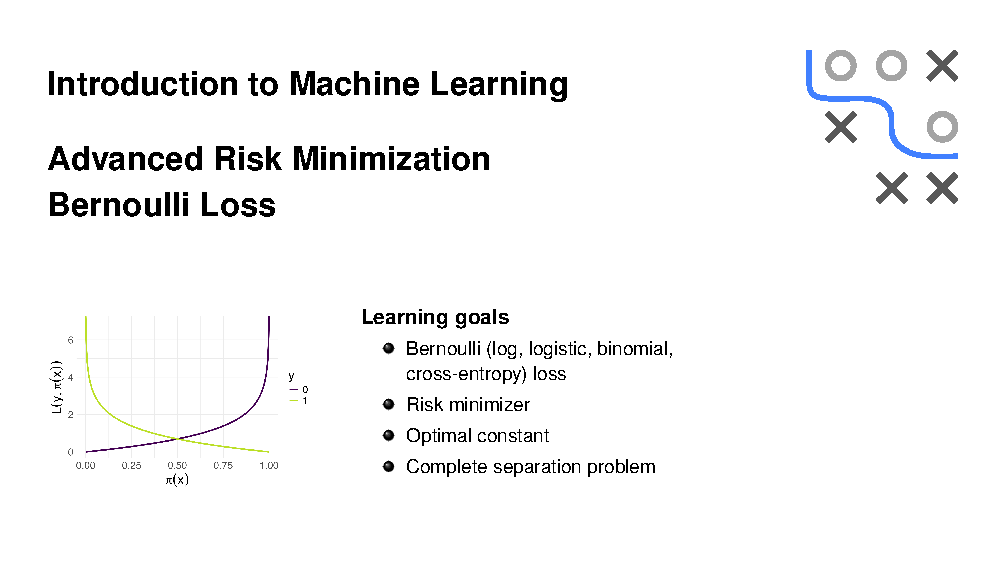
\includepdf[pages=-]{../../slides-pdf/slides-advriskmin-classification-bernoulli.pdf}

\subsection{Some details on classification losses (Deep Dive)}
\includepdf[pages=-]{../../slides-pdf/slides-advriskmin-detailsclassif-deepdive.pdf}

\subsection{Logistic Regression (Deep-Dive)}
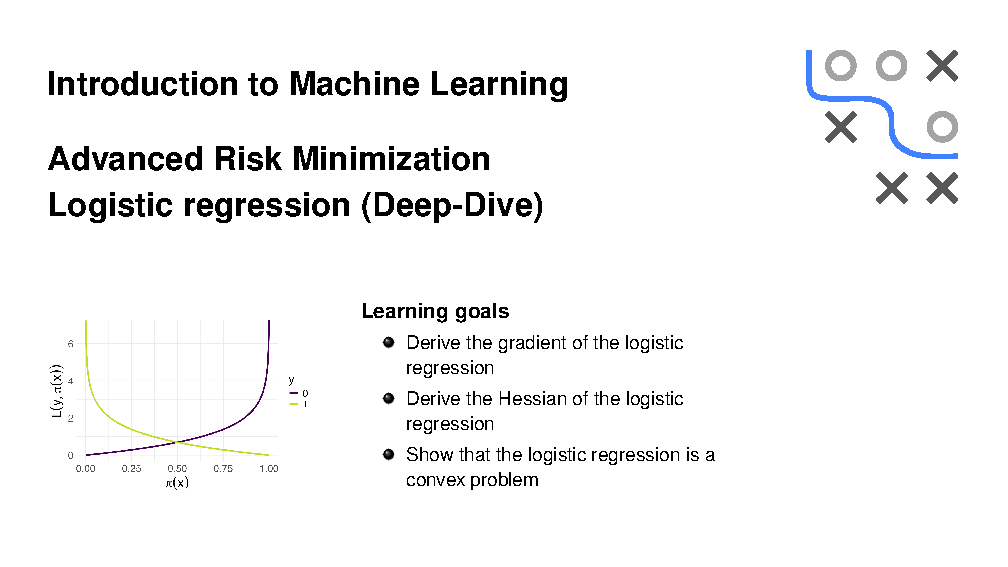
\includepdf[pages=-]{../../slides-pdf/slides-advriskmin-logreg-deepdive.pdf}

\subsection{Brier Score}
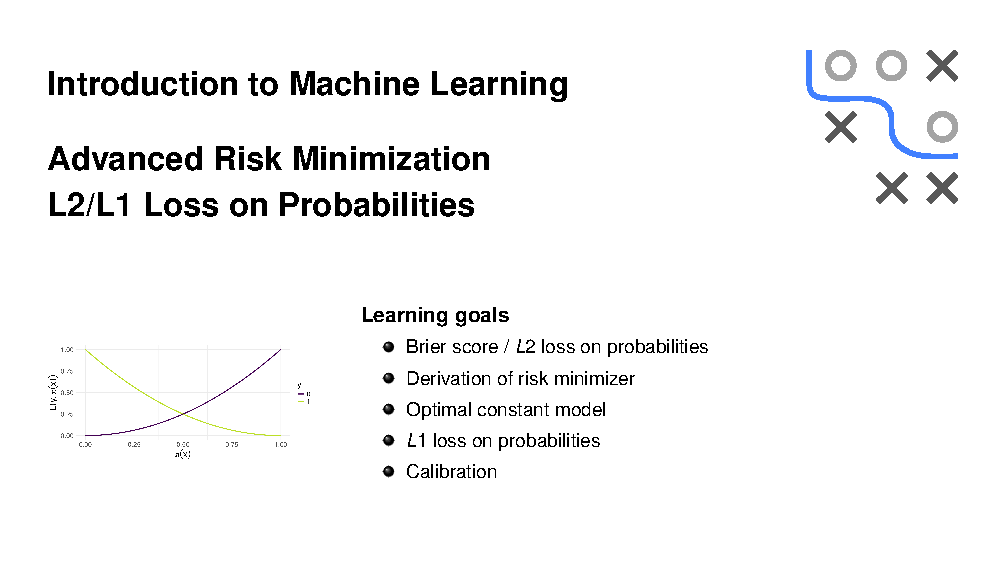
\includepdf[pages=-]{../../slides-pdf/slides-advriskmin-classification-brier-l1.pdf}

\subsection{Advanced Classification Losses}
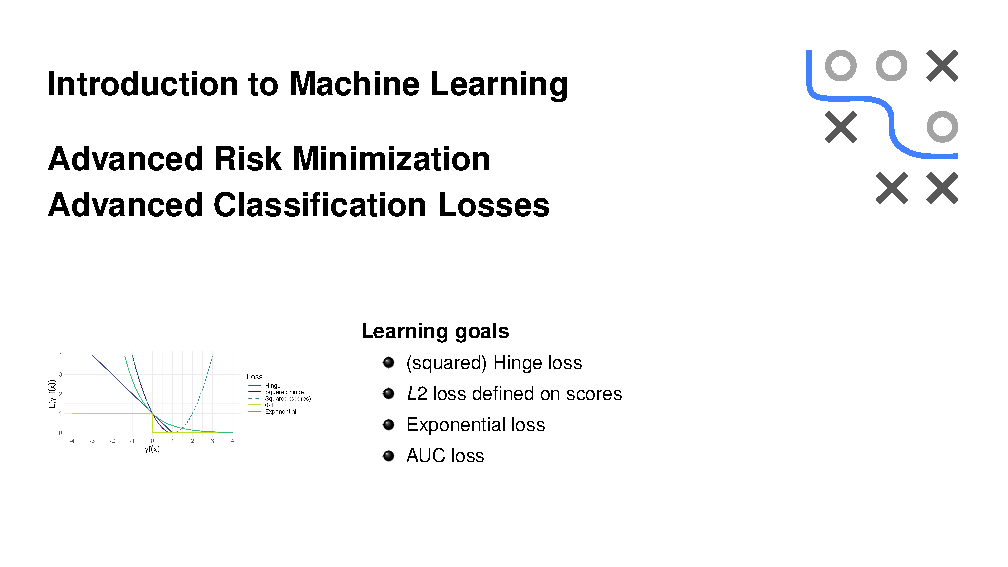
\includepdf[pages=-]{../../slides-pdf/slides-advriskmin-classification-furtherlosses.pdf}

\subsection{Proper Scoring Rules}
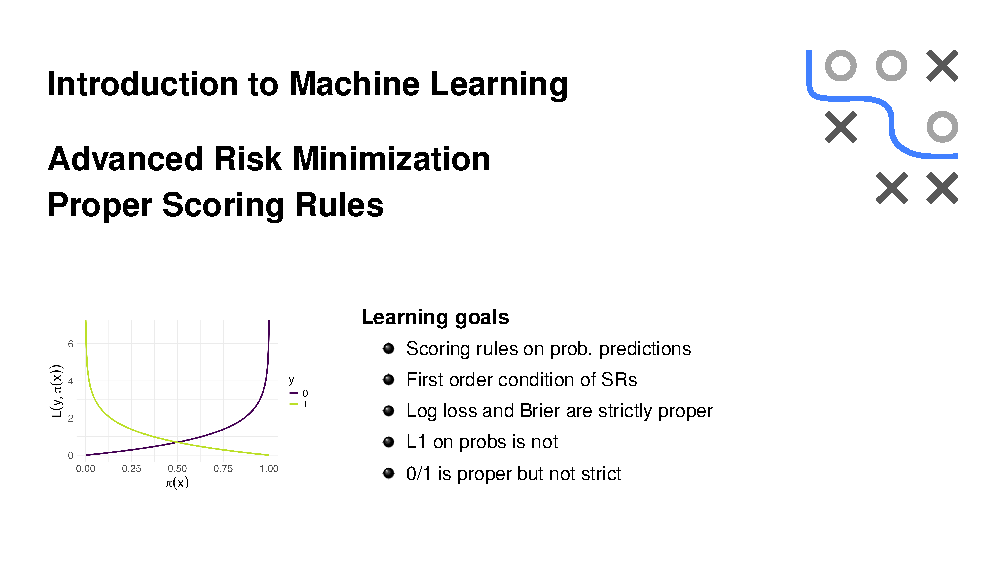
\includepdf[pages=-]{../../slides-pdf/slides-advriskmin-proper-scoring-rules.pdf}

\subsection{Tree Splitting and Loss Functions (Deep-Dive)}
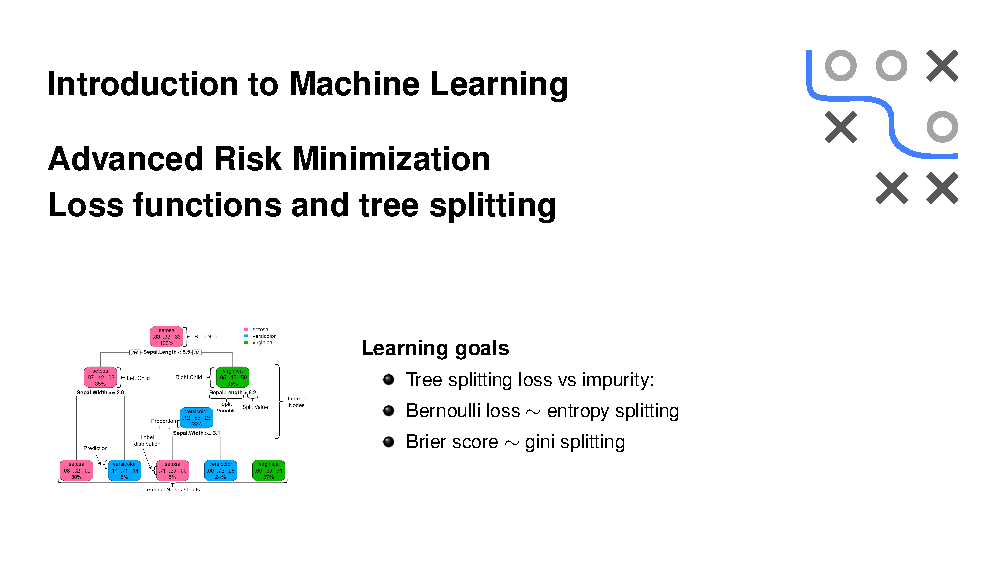
\includepdf[pages=-]{../../slides-pdf/slides-advriskmin-tree-splitting.pdf}
%slides-advriskmin-tree-splitting-deepdive

\subsection{Maximum Likelihood Estimation vs. Empirical Risk Minimization}
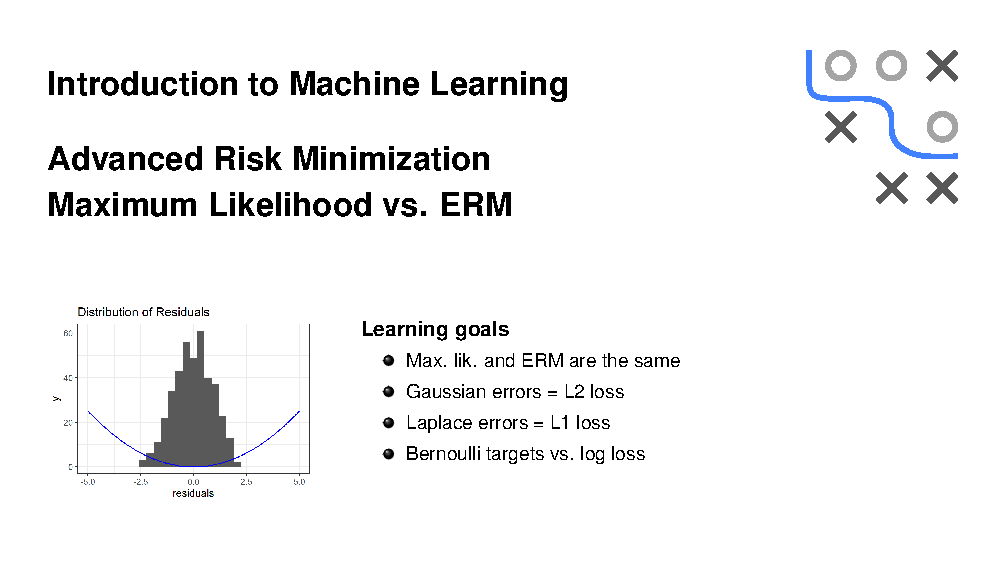
\includepdf[pages=-]{../../slides-pdf/slides-advriskmin-max-likelihood.pdf}

\subsection{Bias Variance Decomposition I}
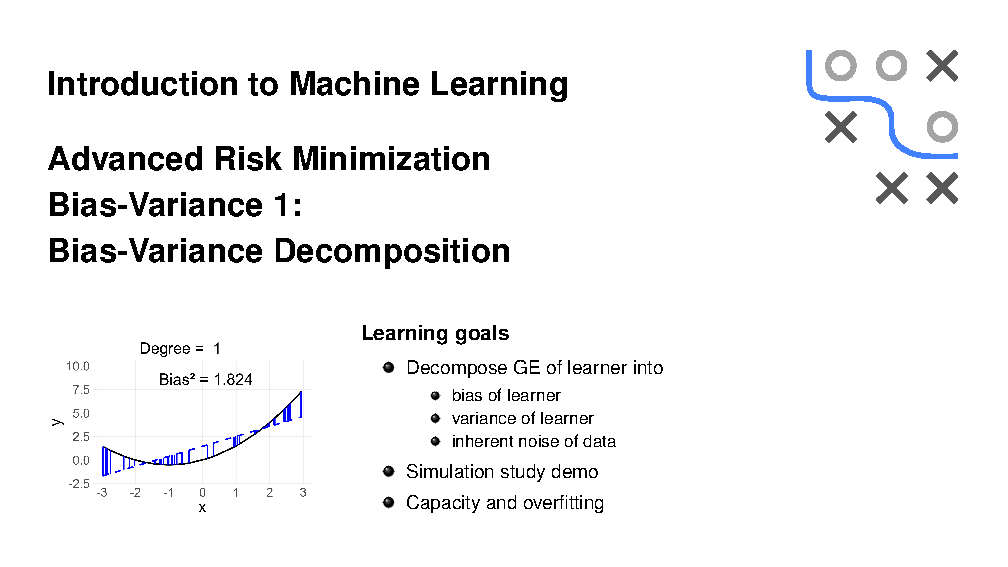
\includepdf[pages=-]{../../slides-pdf/slides-advriskmin-bias-variance-decomposition-1.pdf}

\subsection{Bias Variance Decomposition II}
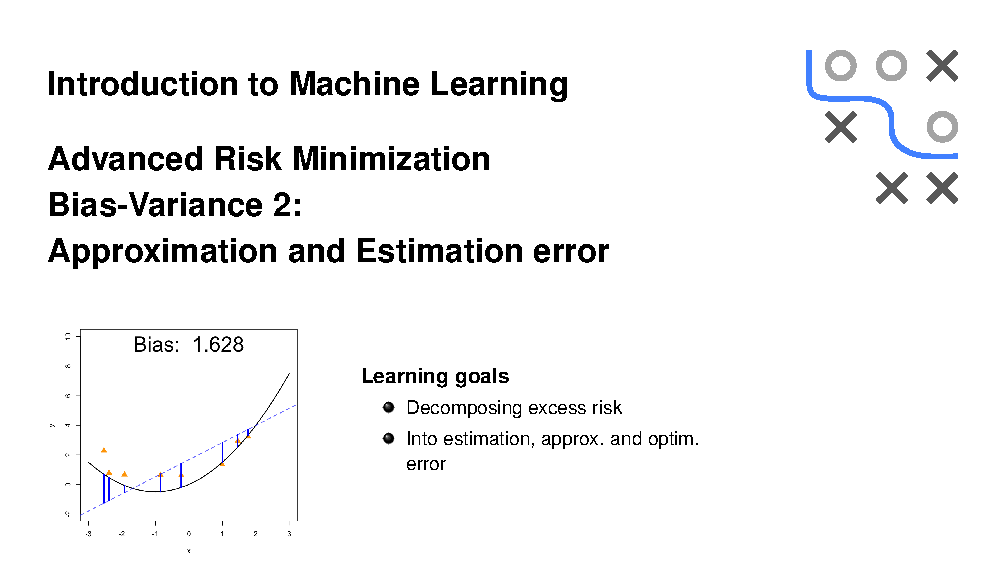
\includepdf[pages=-]{../../slides-pdf/slides-advriskmin-bias-variance-decomposition-2.pdf}

\subsection{Bias Variance Decomposition (Deep-Dive)}
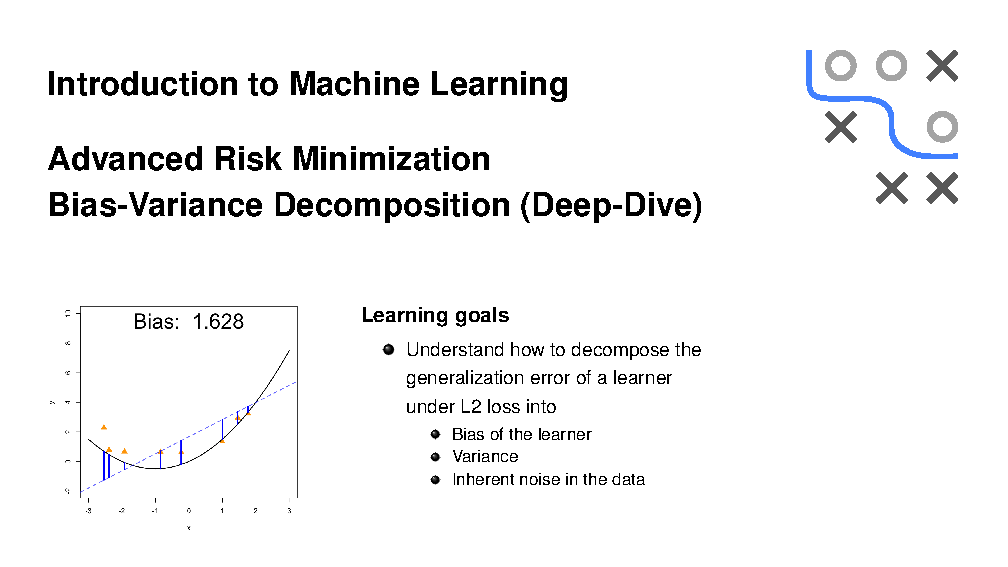
\includepdf[pages=-]{../../slides-pdf/slides-advriskmin-bias-variance-decomposition-deepdive.pdf}




\section{Multiclass Classification}
\subsection{Risk Minimization Basics}
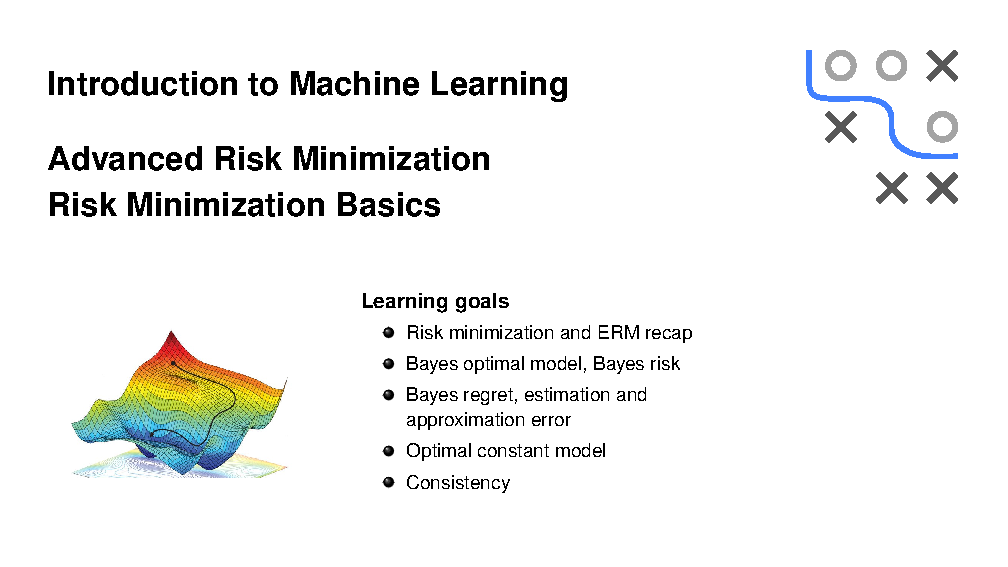
\includepdf[pages=-]{../../slides-pdf/slides-advriskmin-risk-minimization-basics.pdf}

\subsection{Loss Properties}
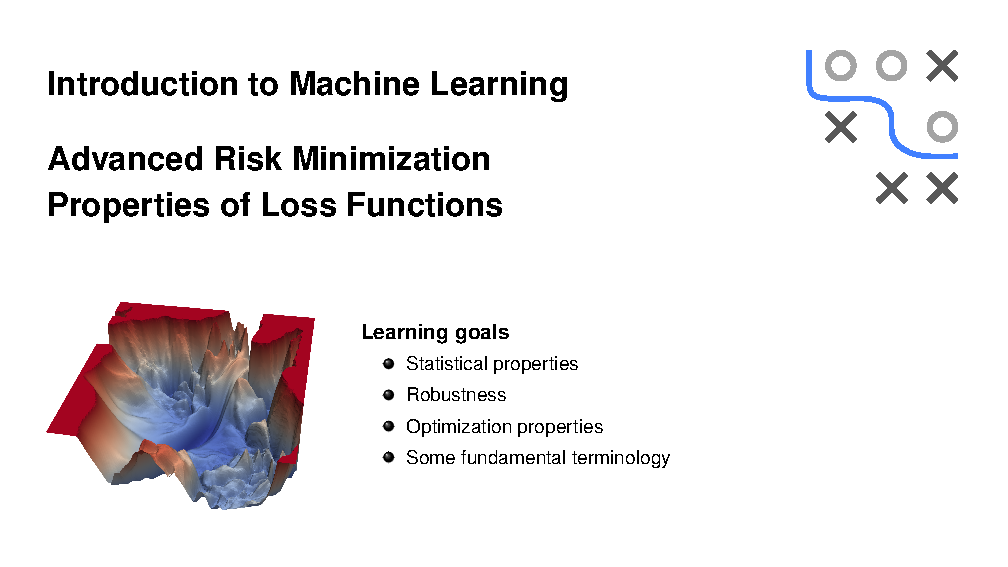
\includepdf[pages=-]{../../slides-pdf/slides-advriskmin-losses-properties.pdf}

\subsection{Pseudo-Residuals}
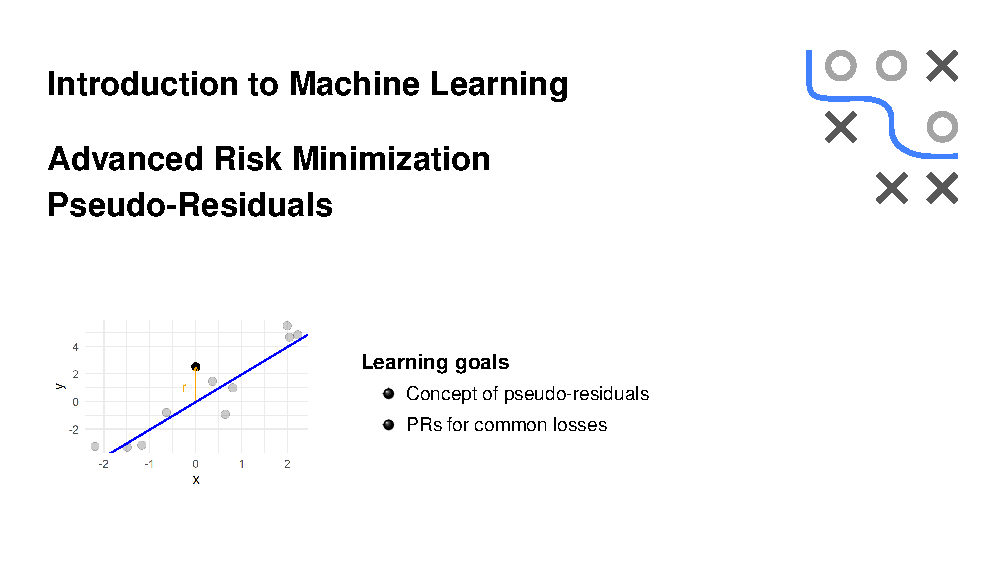
\includepdf[pages=-]{../../slides-pdf/slides-advriskmin-pseudo-residuals.pdf}

\subsection{L2- and L1-loss}
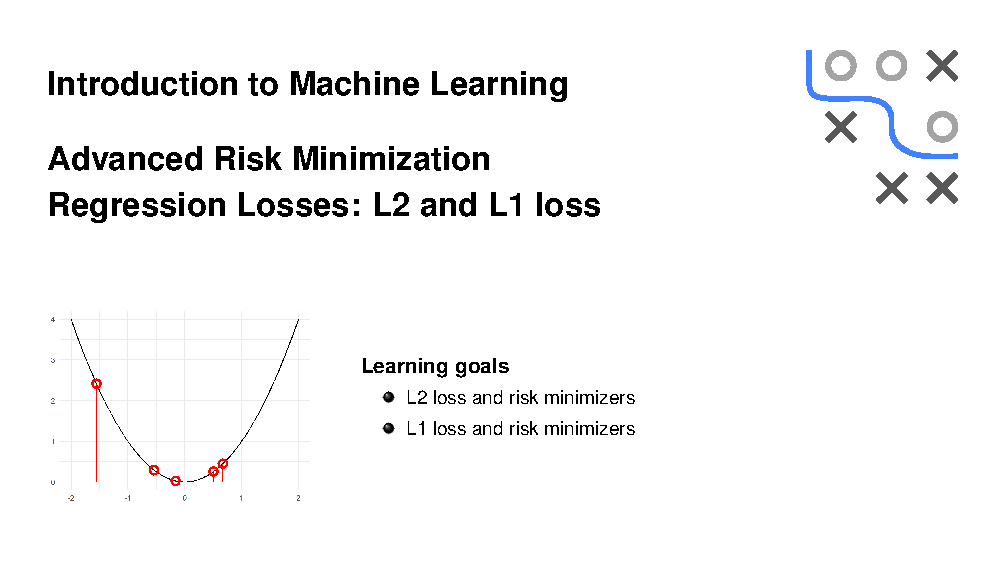
\includepdf[pages=-]{../../slides-pdf/slides-advriskmin-regression-l2-l1.pdf}

\subsection{L1 Risk Minimizer (Deep-Dive)}
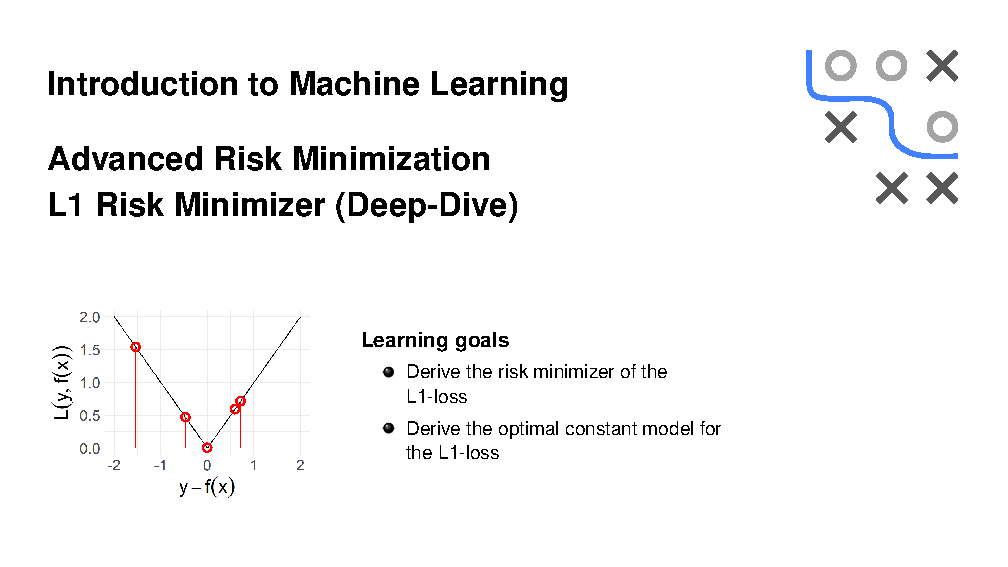
\includepdf[pages=-]{../../slides-pdf/slides-advriskmin-regression-l1-deepdive.pdf}

\subsection{Advanced Regression Losses}
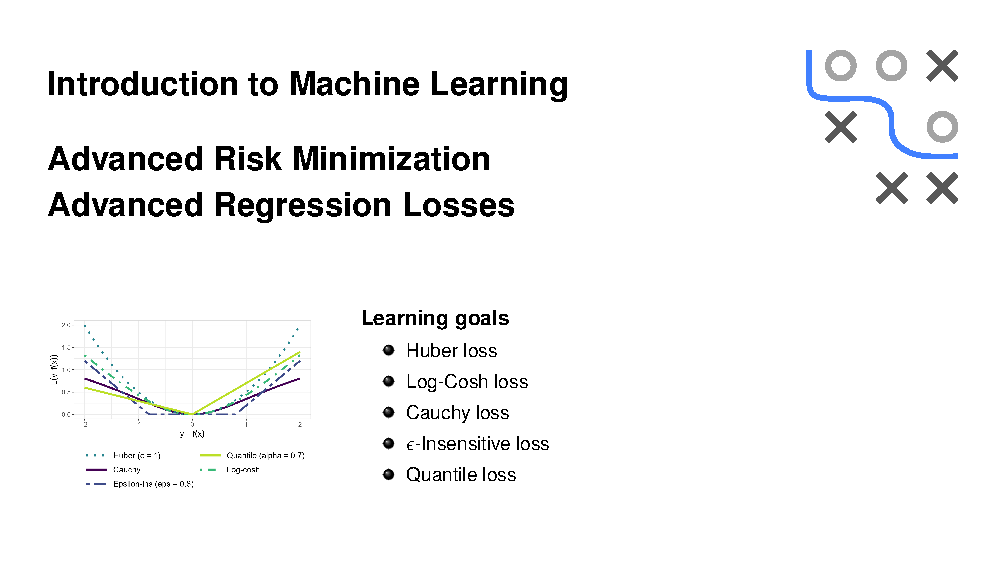
\includepdf[pages=-]{../../slides-pdf/slides-advriskmin-regression-further-losses.pdf}

\subsection{0-1-loss}
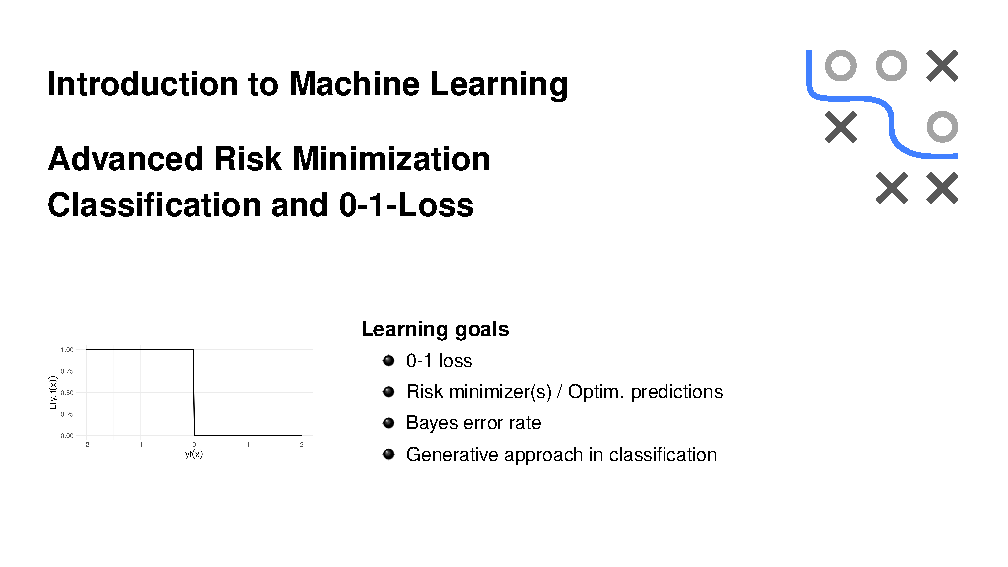
\includepdf[pages=-]{../../slides-pdf/slides-advriskmin-classification-01.pdf}

\subsection{Bernoulli Loss}
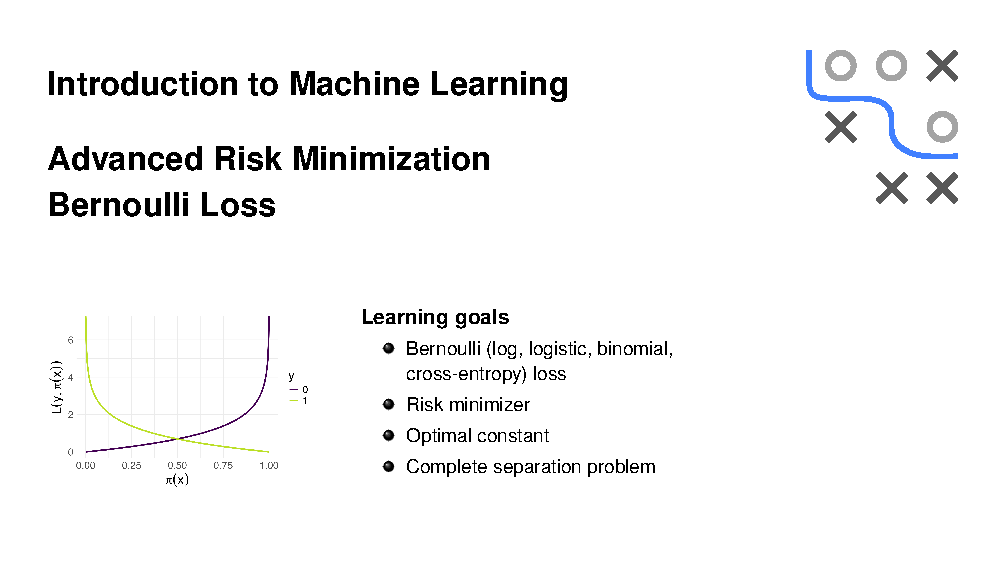
\includepdf[pages=-]{../../slides-pdf/slides-advriskmin-classification-bernoulli.pdf}

\subsection{Some details on classification losses (Deep Dive)}
\includepdf[pages=-]{../../slides-pdf/slides-advriskmin-detailsclassif-deepdive.pdf}

\subsection{Logistic Regression (Deep-Dive)}
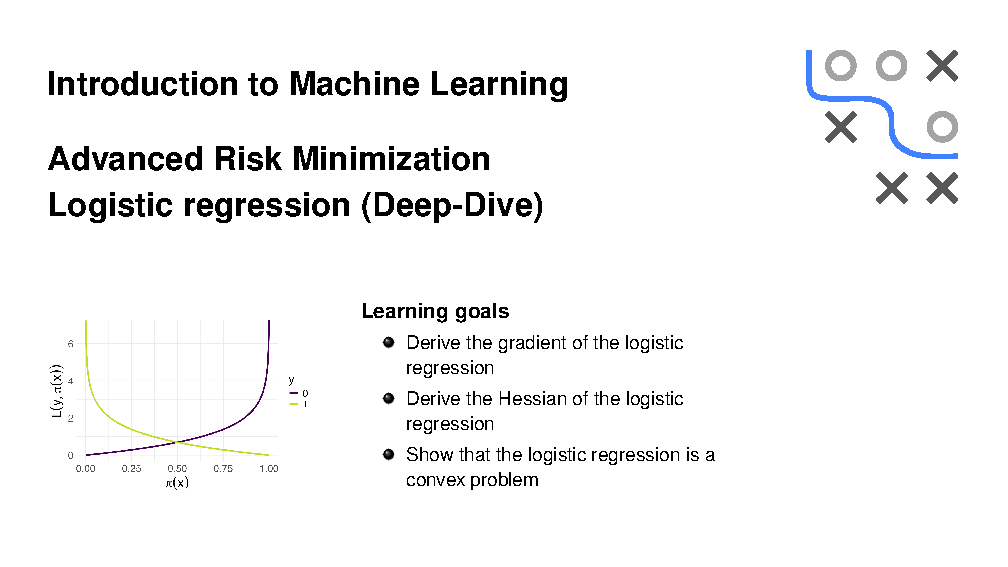
\includepdf[pages=-]{../../slides-pdf/slides-advriskmin-logreg-deepdive.pdf}

\subsection{Brier Score}
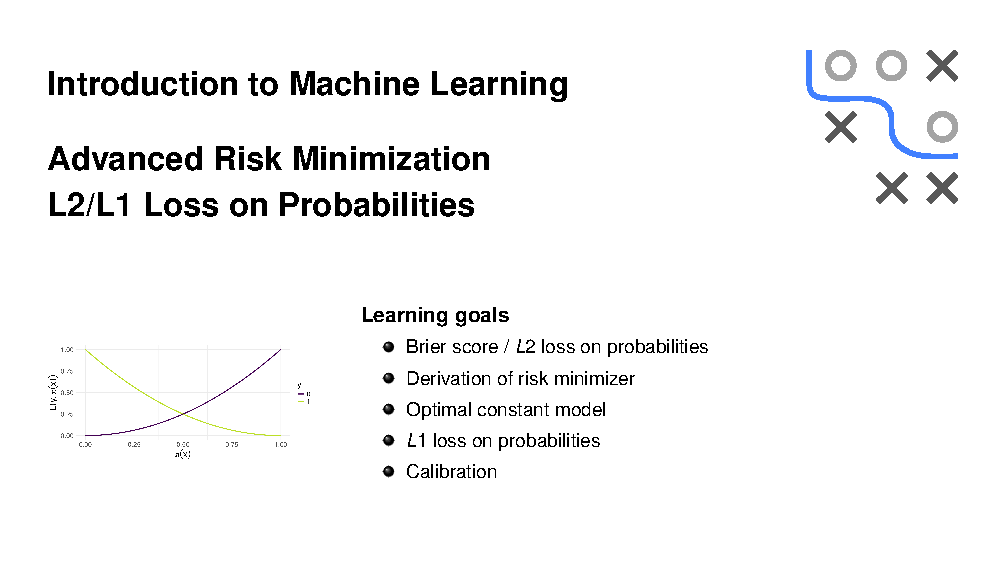
\includepdf[pages=-]{../../slides-pdf/slides-advriskmin-classification-brier-l1.pdf}

\subsection{Advanced Classification Losses}
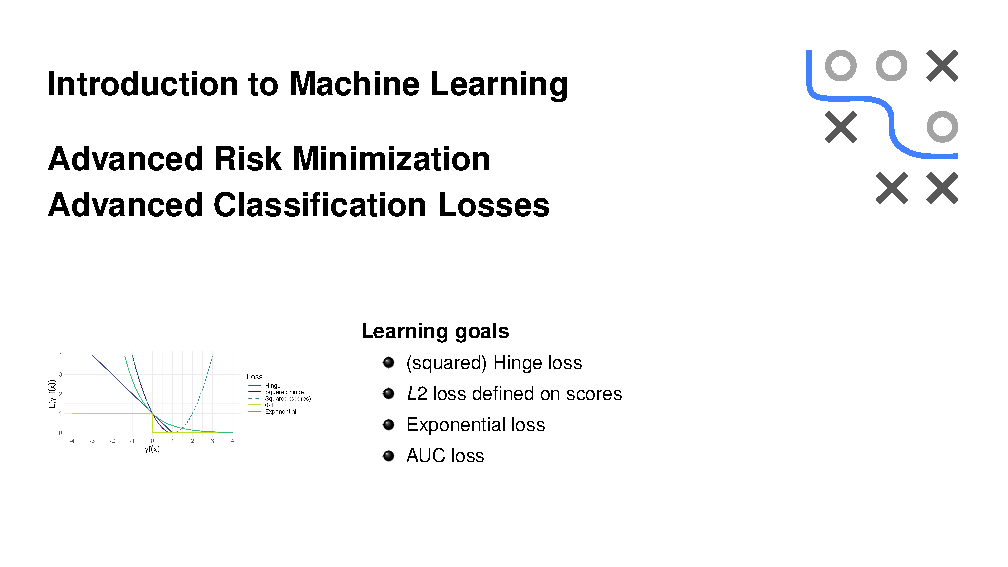
\includepdf[pages=-]{../../slides-pdf/slides-advriskmin-classification-furtherlosses.pdf}

\subsection{Proper Scoring Rules}
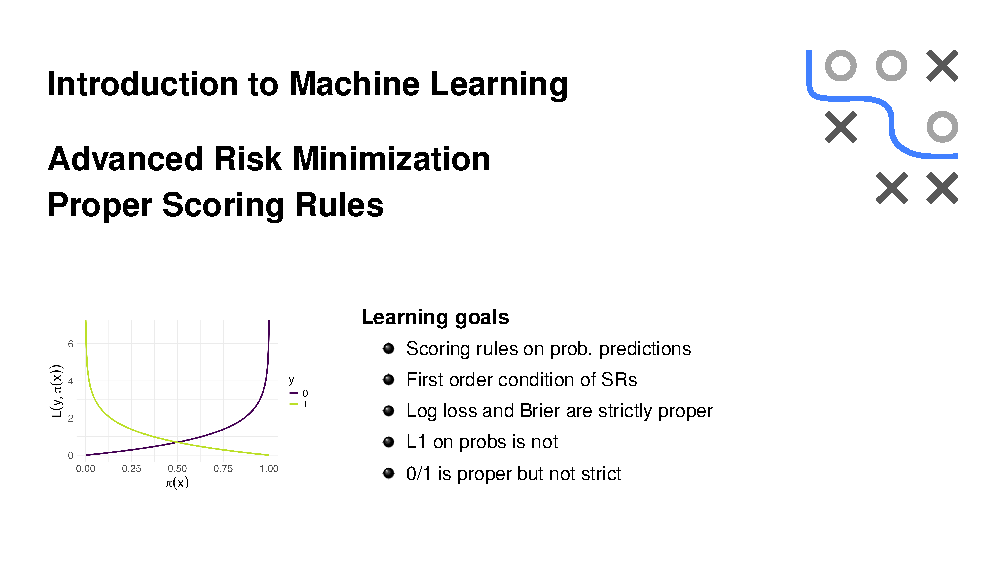
\includepdf[pages=-]{../../slides-pdf/slides-advriskmin-proper-scoring-rules.pdf}

\subsection{Tree Splitting and Loss Functions (Deep-Dive)}
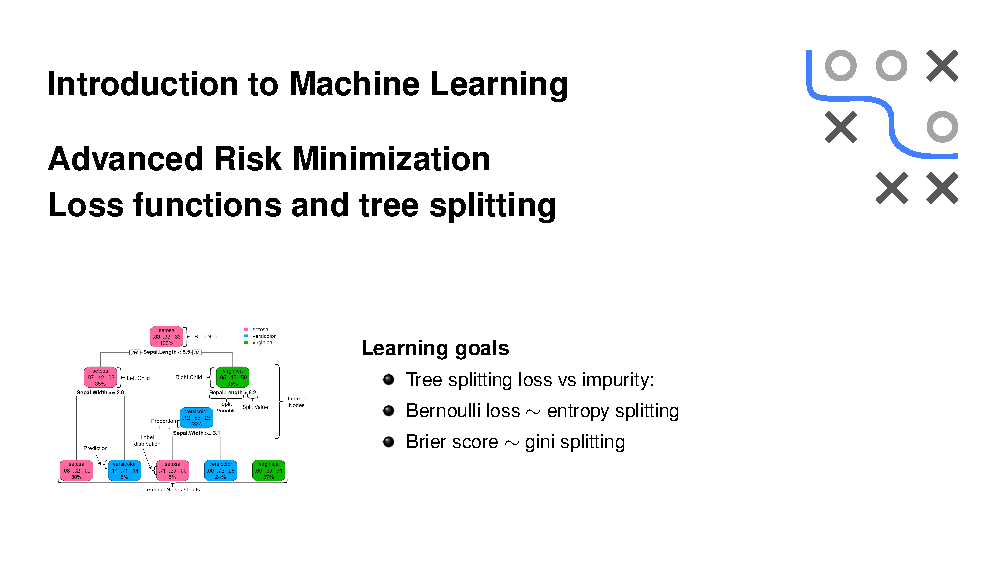
\includepdf[pages=-]{../../slides-pdf/slides-advriskmin-tree-splitting.pdf}
%slides-advriskmin-tree-splitting-deepdive

\subsection{Maximum Likelihood Estimation vs. Empirical Risk Minimization}
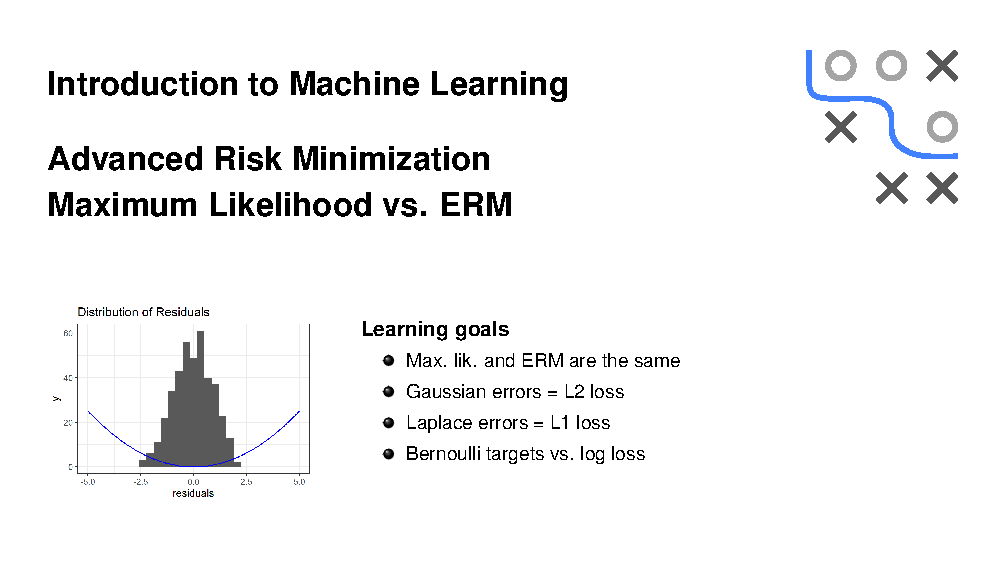
\includepdf[pages=-]{../../slides-pdf/slides-advriskmin-max-likelihood.pdf}

\subsection{Bias Variance Decomposition I}
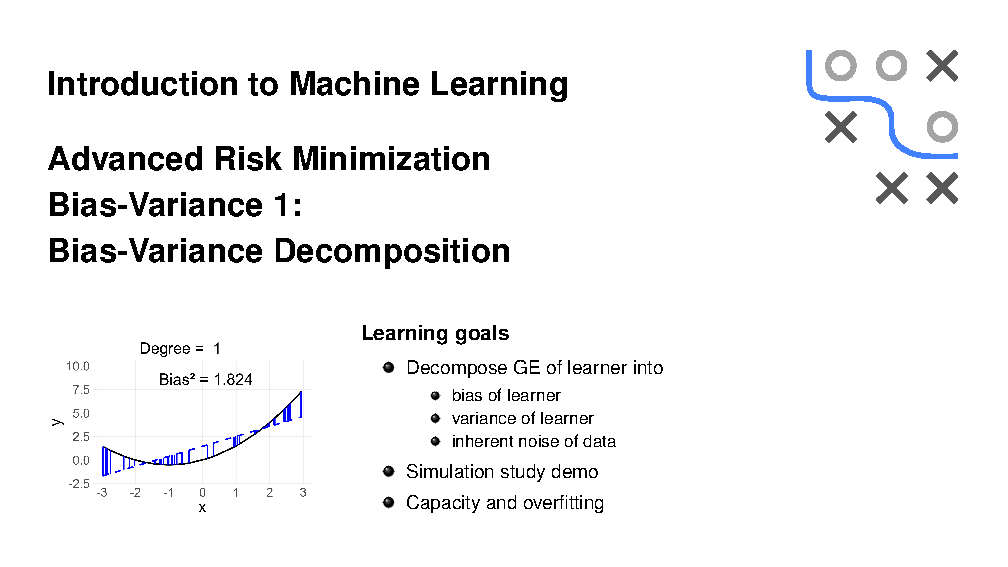
\includepdf[pages=-]{../../slides-pdf/slides-advriskmin-bias-variance-decomposition-1.pdf}

\subsection{Bias Variance Decomposition II}
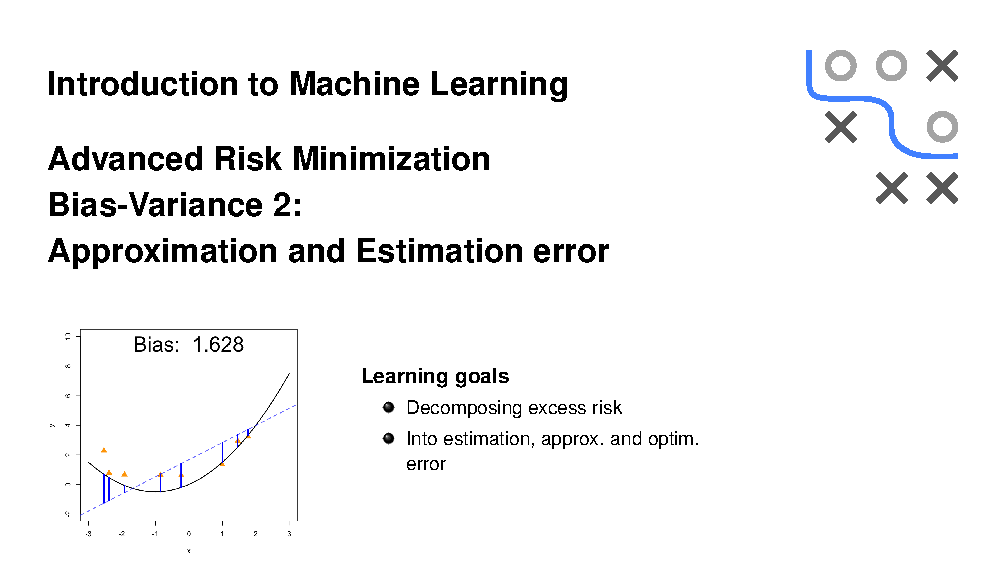
\includepdf[pages=-]{../../slides-pdf/slides-advriskmin-bias-variance-decomposition-2.pdf}

\subsection{Bias Variance Decomposition (Deep-Dive)}
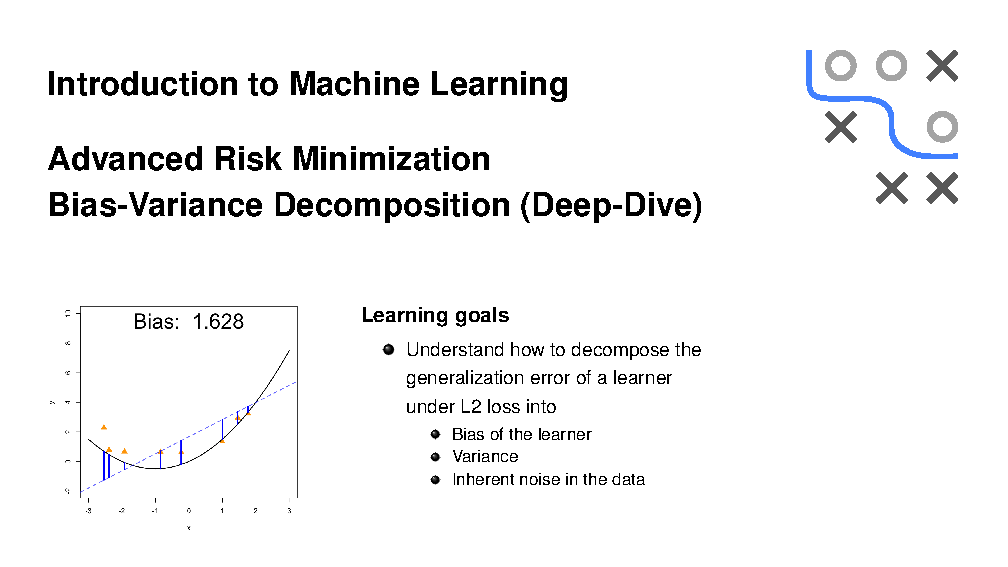
\includepdf[pages=-]{../../slides-pdf/slides-advriskmin-bias-variance-decomposition-deepdive.pdf}




\section{Information Theory}
\subsection{Risk Minimization Basics}
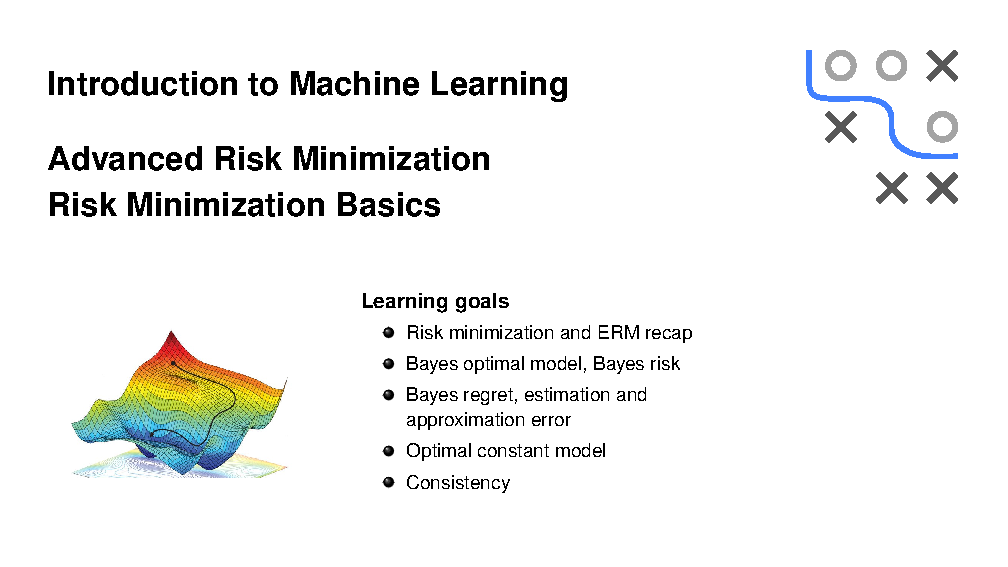
\includepdf[pages=-]{../../slides-pdf/slides-advriskmin-risk-minimization-basics.pdf}

\subsection{Loss Properties}
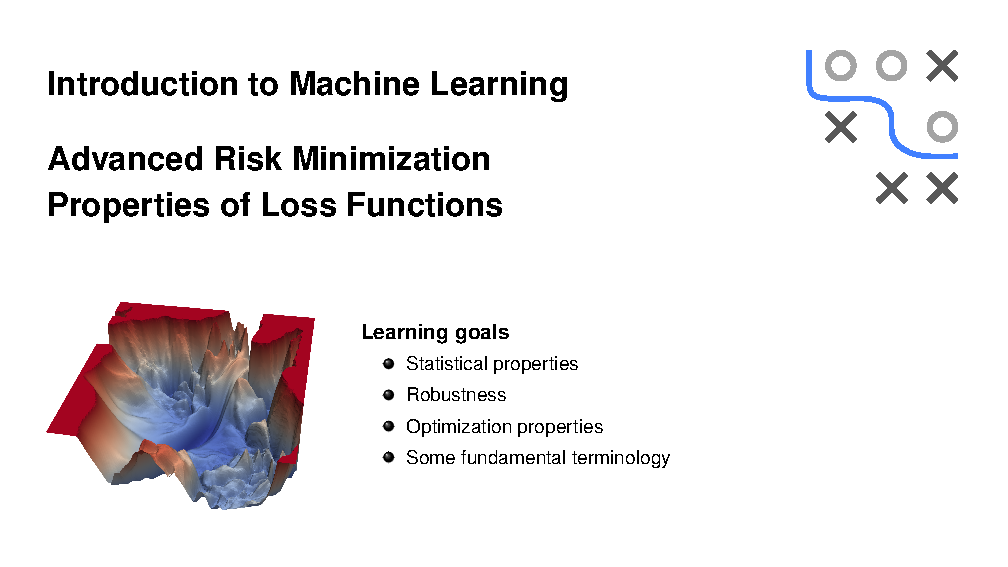
\includepdf[pages=-]{../../slides-pdf/slides-advriskmin-losses-properties.pdf}

\subsection{Pseudo-Residuals}
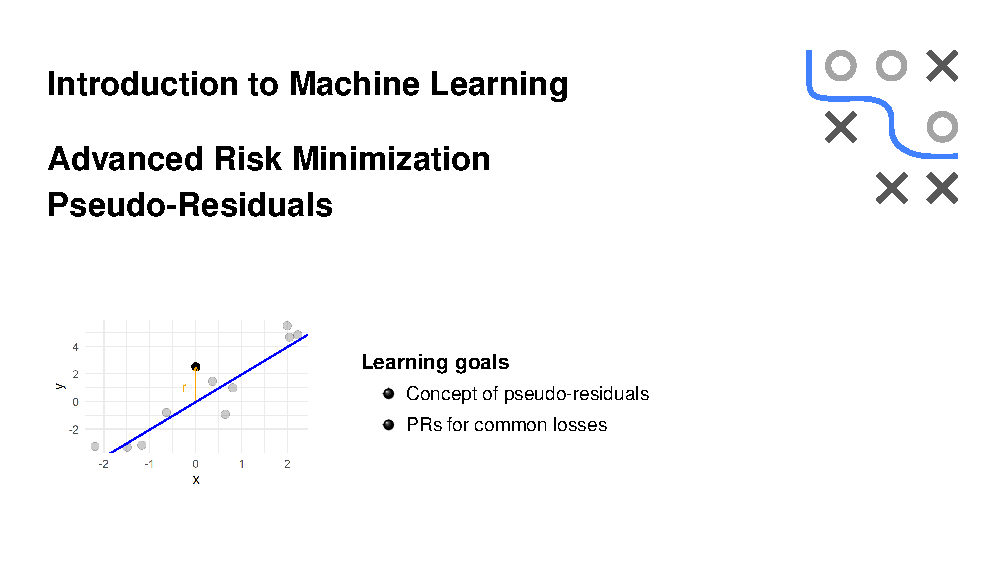
\includepdf[pages=-]{../../slides-pdf/slides-advriskmin-pseudo-residuals.pdf}

\subsection{L2- and L1-loss}
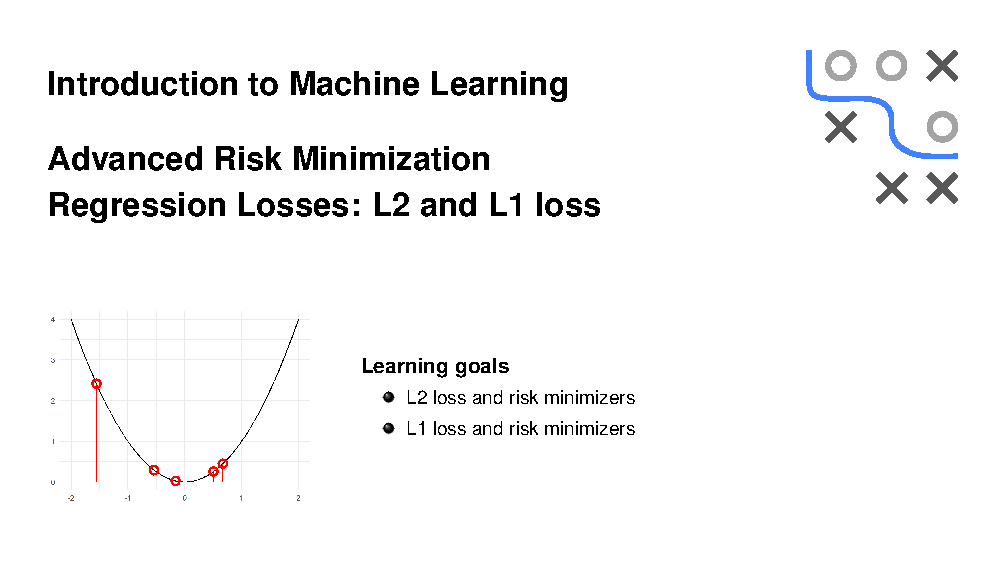
\includepdf[pages=-]{../../slides-pdf/slides-advriskmin-regression-l2-l1.pdf}

\subsection{L1 Risk Minimizer (Deep-Dive)}
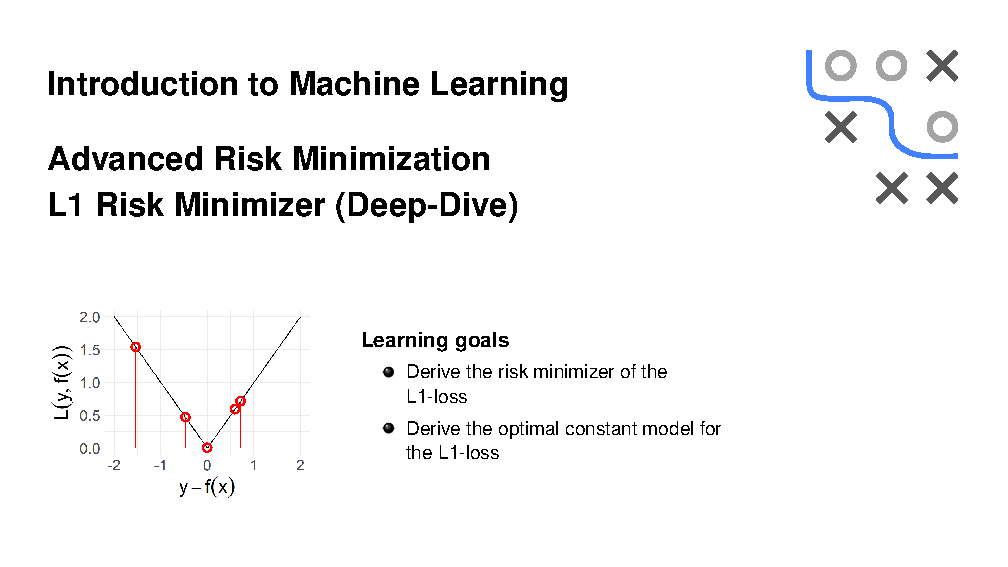
\includepdf[pages=-]{../../slides-pdf/slides-advriskmin-regression-l1-deepdive.pdf}

\subsection{Advanced Regression Losses}
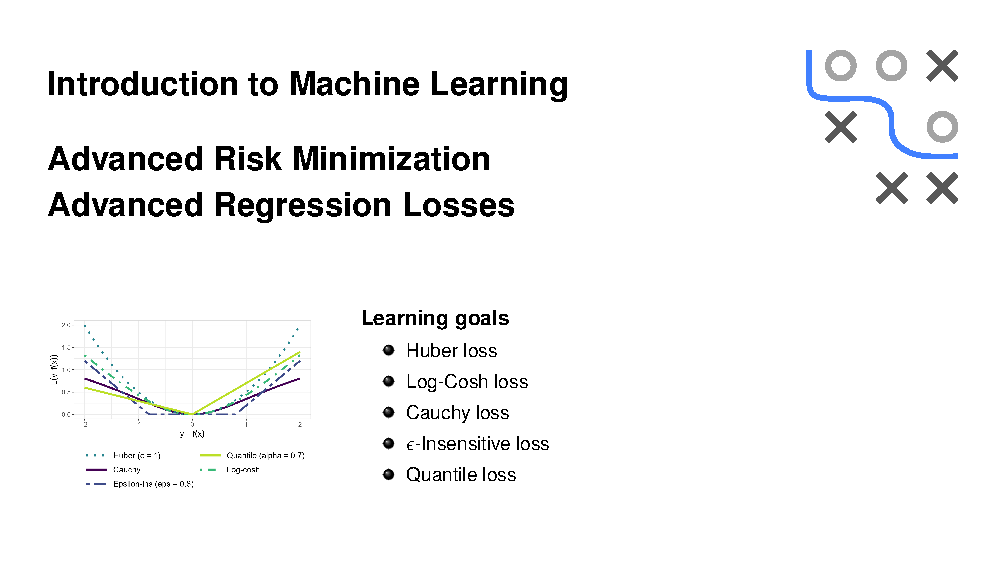
\includepdf[pages=-]{../../slides-pdf/slides-advriskmin-regression-further-losses.pdf}

\subsection{0-1-loss}
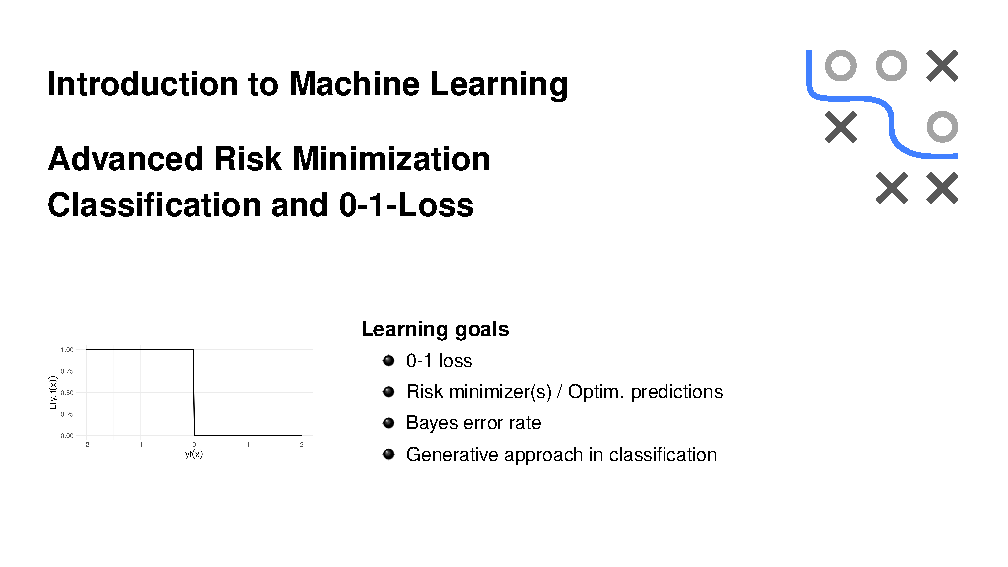
\includepdf[pages=-]{../../slides-pdf/slides-advriskmin-classification-01.pdf}

\subsection{Bernoulli Loss}
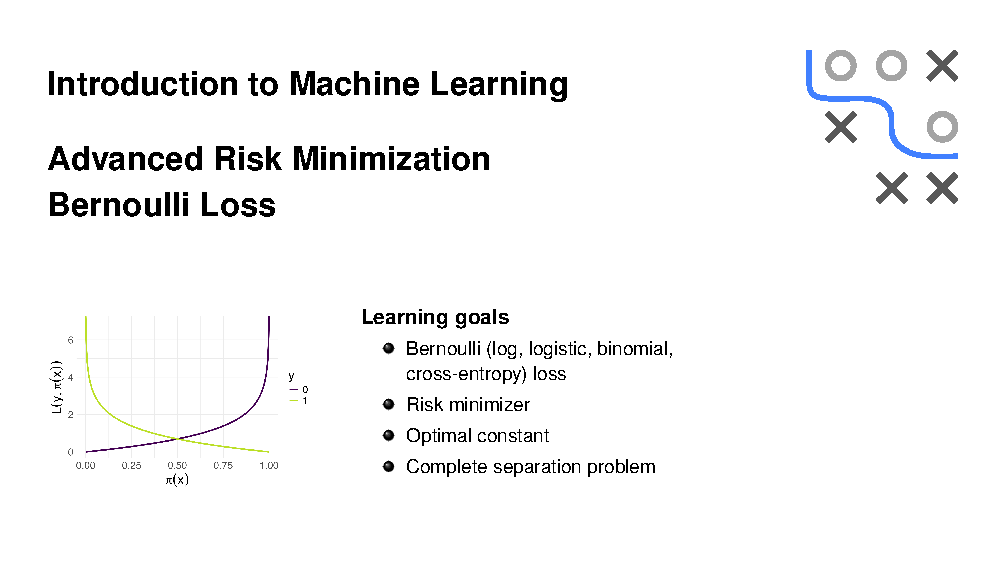
\includepdf[pages=-]{../../slides-pdf/slides-advriskmin-classification-bernoulli.pdf}

\subsection{Some details on classification losses (Deep Dive)}
\includepdf[pages=-]{../../slides-pdf/slides-advriskmin-detailsclassif-deepdive.pdf}

\subsection{Logistic Regression (Deep-Dive)}
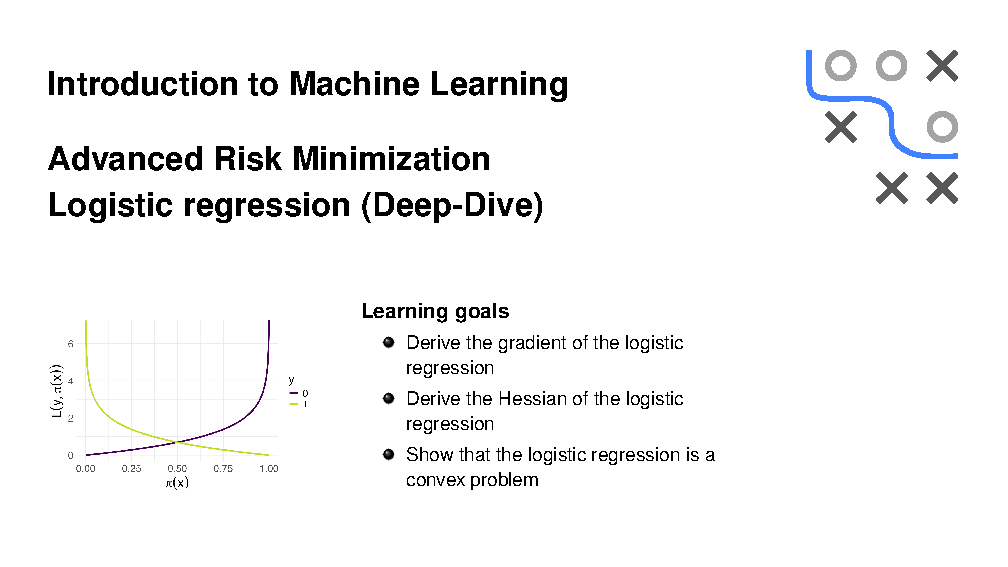
\includepdf[pages=-]{../../slides-pdf/slides-advriskmin-logreg-deepdive.pdf}

\subsection{Brier Score}
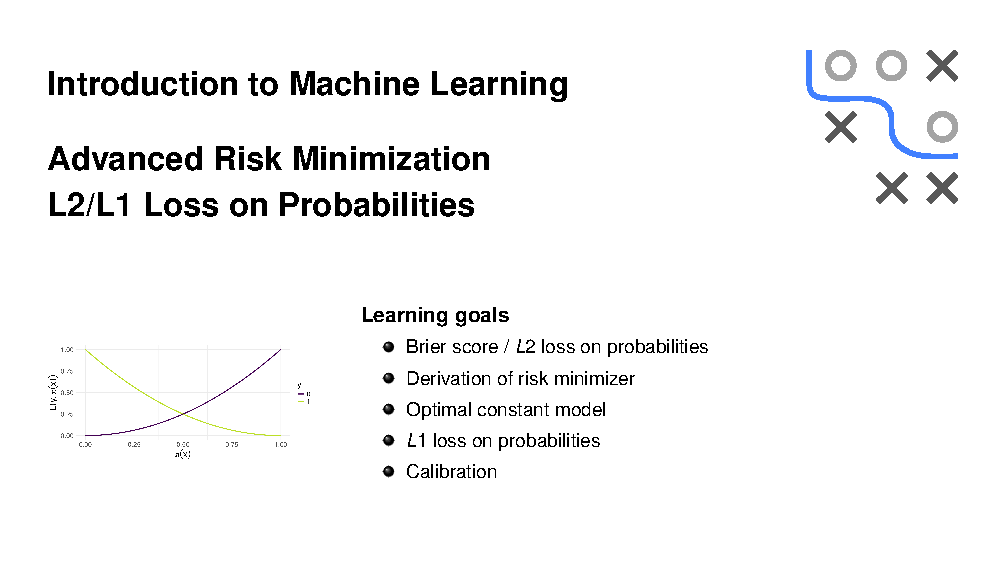
\includepdf[pages=-]{../../slides-pdf/slides-advriskmin-classification-brier-l1.pdf}

\subsection{Advanced Classification Losses}
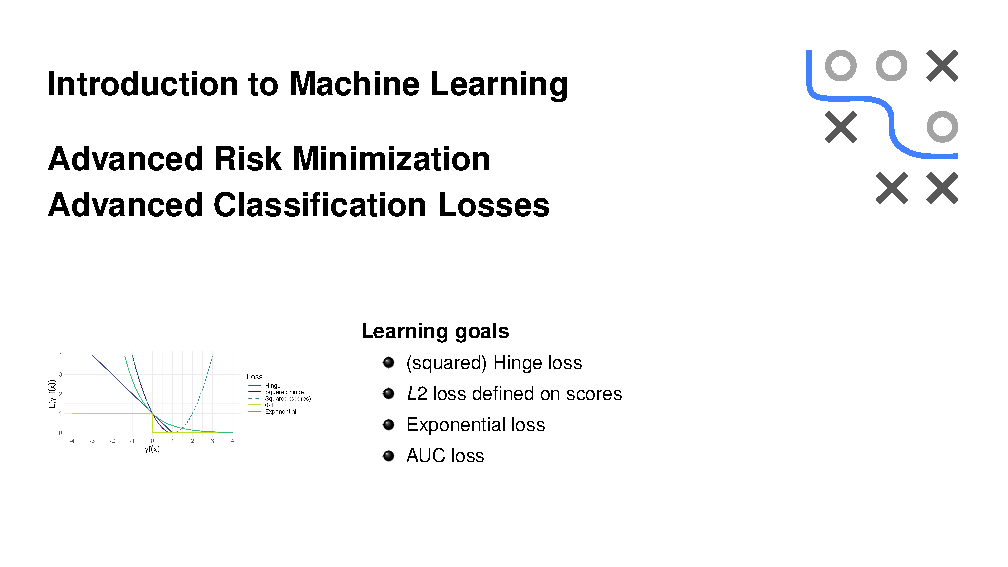
\includepdf[pages=-]{../../slides-pdf/slides-advriskmin-classification-furtherlosses.pdf}

\subsection{Proper Scoring Rules}
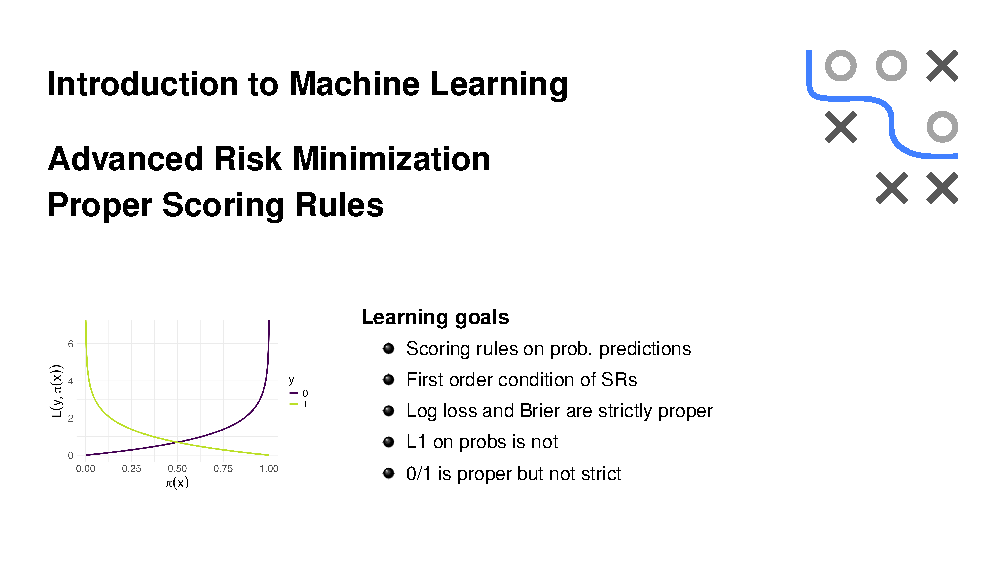
\includepdf[pages=-]{../../slides-pdf/slides-advriskmin-proper-scoring-rules.pdf}

\subsection{Tree Splitting and Loss Functions (Deep-Dive)}
\includepdf[pages=-]{../../slides-pdf/slides-advriskmin-tree-splitting.pdf}
%slides-advriskmin-tree-splitting-deepdive

\subsection{Maximum Likelihood Estimation vs. Empirical Risk Minimization}
\includepdf[pages=-]{../../slides-pdf/slides-advriskmin-max-likelihood.pdf}

\subsection{Bias Variance Decomposition I}
\includepdf[pages=-]{../../slides-pdf/slides-advriskmin-bias-variance-decomposition-1.pdf}

\subsection{Bias Variance Decomposition II}
\includepdf[pages=-]{../../slides-pdf/slides-advriskmin-bias-variance-decomposition-2.pdf}

\subsection{Bias Variance Decomposition (Deep-Dive)}
\includepdf[pages=-]{../../slides-pdf/slides-advriskmin-bias-variance-decomposition-deepdive.pdf}




\section{Curse of Dimensionality}
\subsection{Risk Minimization Basics}
\includepdf[pages=-]{../../slides-pdf/slides-advriskmin-risk-minimization-basics.pdf}

\subsection{Loss Properties}
\includepdf[pages=-]{../../slides-pdf/slides-advriskmin-losses-properties.pdf}

\subsection{Pseudo-Residuals}
\includepdf[pages=-]{../../slides-pdf/slides-advriskmin-pseudo-residuals.pdf}

\subsection{L2- and L1-loss}
\includepdf[pages=-]{../../slides-pdf/slides-advriskmin-regression-l2-l1.pdf}

\subsection{L1 Risk Minimizer (Deep-Dive)}
\includepdf[pages=-]{../../slides-pdf/slides-advriskmin-regression-l1-deepdive.pdf}

\subsection{Advanced Regression Losses}
\includepdf[pages=-]{../../slides-pdf/slides-advriskmin-regression-further-losses.pdf}

\subsection{0-1-loss}
\includepdf[pages=-]{../../slides-pdf/slides-advriskmin-classification-01.pdf}

\subsection{Bernoulli Loss}
\includepdf[pages=-]{../../slides-pdf/slides-advriskmin-classification-bernoulli.pdf}

\subsection{Some details on classification losses (Deep Dive)}
\includepdf[pages=-]{../../slides-pdf/slides-advriskmin-detailsclassif-deepdive.pdf}

\subsection{Logistic Regression (Deep-Dive)}
\includepdf[pages=-]{../../slides-pdf/slides-advriskmin-logreg-deepdive.pdf}

\subsection{Brier Score}
\includepdf[pages=-]{../../slides-pdf/slides-advriskmin-classification-brier-l1.pdf}

\subsection{Advanced Classification Losses}
\includepdf[pages=-]{../../slides-pdf/slides-advriskmin-classification-furtherlosses.pdf}

\subsection{Proper Scoring Rules}
\includepdf[pages=-]{../../slides-pdf/slides-advriskmin-proper-scoring-rules.pdf}

\subsection{Tree Splitting and Loss Functions (Deep-Dive)}
\includepdf[pages=-]{../../slides-pdf/slides-advriskmin-tree-splitting.pdf}
%slides-advriskmin-tree-splitting-deepdive

\subsection{Maximum Likelihood Estimation vs. Empirical Risk Minimization}
\includepdf[pages=-]{../../slides-pdf/slides-advriskmin-max-likelihood.pdf}

\subsection{Bias Variance Decomposition I}
\includepdf[pages=-]{../../slides-pdf/slides-advriskmin-bias-variance-decomposition-1.pdf}

\subsection{Bias Variance Decomposition II}
\includepdf[pages=-]{../../slides-pdf/slides-advriskmin-bias-variance-decomposition-2.pdf}

\subsection{Bias Variance Decomposition (Deep-Dive)}
\includepdf[pages=-]{../../slides-pdf/slides-advriskmin-bias-variance-decomposition-deepdive.pdf}




%\section{Hypothesis Space}
%\subsection{Risk Minimization Basics}
\includepdf[pages=-]{../../slides-pdf/slides-advriskmin-risk-minimization-basics.pdf}

\subsection{Loss Properties}
\includepdf[pages=-]{../../slides-pdf/slides-advriskmin-losses-properties.pdf}

\subsection{Pseudo-Residuals}
\includepdf[pages=-]{../../slides-pdf/slides-advriskmin-pseudo-residuals.pdf}

\subsection{L2- and L1-loss}
\includepdf[pages=-]{../../slides-pdf/slides-advriskmin-regression-l2-l1.pdf}

\subsection{L1 Risk Minimizer (Deep-Dive)}
\includepdf[pages=-]{../../slides-pdf/slides-advriskmin-regression-l1-deepdive.pdf}

\subsection{Advanced Regression Losses}
\includepdf[pages=-]{../../slides-pdf/slides-advriskmin-regression-further-losses.pdf}

\subsection{0-1-loss}
\includepdf[pages=-]{../../slides-pdf/slides-advriskmin-classification-01.pdf}

\subsection{Bernoulli Loss}
\includepdf[pages=-]{../../slides-pdf/slides-advriskmin-classification-bernoulli.pdf}

\subsection{Some details on classification losses (Deep Dive)}
\includepdf[pages=-]{../../slides-pdf/slides-advriskmin-detailsclassif-deepdive.pdf}

\subsection{Logistic Regression (Deep-Dive)}
\includepdf[pages=-]{../../slides-pdf/slides-advriskmin-logreg-deepdive.pdf}

\subsection{Brier Score}
\includepdf[pages=-]{../../slides-pdf/slides-advriskmin-classification-brier-l1.pdf}

\subsection{Advanced Classification Losses}
\includepdf[pages=-]{../../slides-pdf/slides-advriskmin-classification-furtherlosses.pdf}

\subsection{Proper Scoring Rules}
\includepdf[pages=-]{../../slides-pdf/slides-advriskmin-proper-scoring-rules.pdf}

\subsection{Tree Splitting and Loss Functions (Deep-Dive)}
\includepdf[pages=-]{../../slides-pdf/slides-advriskmin-tree-splitting.pdf}
%slides-advriskmin-tree-splitting-deepdive

\subsection{Maximum Likelihood Estimation vs. Empirical Risk Minimization}
\includepdf[pages=-]{../../slides-pdf/slides-advriskmin-max-likelihood.pdf}

\subsection{Bias Variance Decomposition I}
\includepdf[pages=-]{../../slides-pdf/slides-advriskmin-bias-variance-decomposition-1.pdf}

\subsection{Bias Variance Decomposition II}
\includepdf[pages=-]{../../slides-pdf/slides-advriskmin-bias-variance-decomposition-2.pdf}

\subsection{Bias Variance Decomposition (Deep-Dive)}
\includepdf[pages=-]{../../slides-pdf/slides-advriskmin-bias-variance-decomposition-deepdive.pdf}




\section{Regularization}
\subsection{Risk Minimization Basics}
\includepdf[pages=-]{../../slides-pdf/slides-advriskmin-risk-minimization-basics.pdf}

\subsection{Loss Properties}
\includepdf[pages=-]{../../slides-pdf/slides-advriskmin-losses-properties.pdf}

\subsection{Pseudo-Residuals}
\includepdf[pages=-]{../../slides-pdf/slides-advriskmin-pseudo-residuals.pdf}

\subsection{L2- and L1-loss}
\includepdf[pages=-]{../../slides-pdf/slides-advriskmin-regression-l2-l1.pdf}

\subsection{L1 Risk Minimizer (Deep-Dive)}
\includepdf[pages=-]{../../slides-pdf/slides-advriskmin-regression-l1-deepdive.pdf}

\subsection{Advanced Regression Losses}
\includepdf[pages=-]{../../slides-pdf/slides-advriskmin-regression-further-losses.pdf}

\subsection{0-1-loss}
\includepdf[pages=-]{../../slides-pdf/slides-advriskmin-classification-01.pdf}

\subsection{Bernoulli Loss}
\includepdf[pages=-]{../../slides-pdf/slides-advriskmin-classification-bernoulli.pdf}

\subsection{Some details on classification losses (Deep Dive)}
\includepdf[pages=-]{../../slides-pdf/slides-advriskmin-detailsclassif-deepdive.pdf}

\subsection{Logistic Regression (Deep-Dive)}
\includepdf[pages=-]{../../slides-pdf/slides-advriskmin-logreg-deepdive.pdf}

\subsection{Brier Score}
\includepdf[pages=-]{../../slides-pdf/slides-advriskmin-classification-brier-l1.pdf}

\subsection{Advanced Classification Losses}
\includepdf[pages=-]{../../slides-pdf/slides-advriskmin-classification-furtherlosses.pdf}

\subsection{Proper Scoring Rules}
\includepdf[pages=-]{../../slides-pdf/slides-advriskmin-proper-scoring-rules.pdf}

\subsection{Tree Splitting and Loss Functions (Deep-Dive)}
\includepdf[pages=-]{../../slides-pdf/slides-advriskmin-tree-splitting.pdf}
%slides-advriskmin-tree-splitting-deepdive

\subsection{Maximum Likelihood Estimation vs. Empirical Risk Minimization}
\includepdf[pages=-]{../../slides-pdf/slides-advriskmin-max-likelihood.pdf}

\subsection{Bias Variance Decomposition I}
\includepdf[pages=-]{../../slides-pdf/slides-advriskmin-bias-variance-decomposition-1.pdf}

\subsection{Bias Variance Decomposition II}
\includepdf[pages=-]{../../slides-pdf/slides-advriskmin-bias-variance-decomposition-2.pdf}

\subsection{Bias Variance Decomposition (Deep-Dive)}
\includepdf[pages=-]{../../slides-pdf/slides-advriskmin-bias-variance-decomposition-deepdive.pdf}




\section{Linear Support Vector Machine}
\subsection{Risk Minimization Basics}
\includepdf[pages=-]{../../slides-pdf/slides-advriskmin-risk-minimization-basics.pdf}

\subsection{Loss Properties}
\includepdf[pages=-]{../../slides-pdf/slides-advriskmin-losses-properties.pdf}

\subsection{Pseudo-Residuals}
\includepdf[pages=-]{../../slides-pdf/slides-advriskmin-pseudo-residuals.pdf}

\subsection{L2- and L1-loss}
\includepdf[pages=-]{../../slides-pdf/slides-advriskmin-regression-l2-l1.pdf}

\subsection{L1 Risk Minimizer (Deep-Dive)}
\includepdf[pages=-]{../../slides-pdf/slides-advriskmin-regression-l1-deepdive.pdf}

\subsection{Advanced Regression Losses}
\includepdf[pages=-]{../../slides-pdf/slides-advriskmin-regression-further-losses.pdf}

\subsection{0-1-loss}
\includepdf[pages=-]{../../slides-pdf/slides-advriskmin-classification-01.pdf}

\subsection{Bernoulli Loss}
\includepdf[pages=-]{../../slides-pdf/slides-advriskmin-classification-bernoulli.pdf}

\subsection{Some details on classification losses (Deep Dive)}
\includepdf[pages=-]{../../slides-pdf/slides-advriskmin-detailsclassif-deepdive.pdf}

\subsection{Logistic Regression (Deep-Dive)}
\includepdf[pages=-]{../../slides-pdf/slides-advriskmin-logreg-deepdive.pdf}

\subsection{Brier Score}
\includepdf[pages=-]{../../slides-pdf/slides-advriskmin-classification-brier-l1.pdf}

\subsection{Advanced Classification Losses}
\includepdf[pages=-]{../../slides-pdf/slides-advriskmin-classification-furtherlosses.pdf}

\subsection{Proper Scoring Rules}
\includepdf[pages=-]{../../slides-pdf/slides-advriskmin-proper-scoring-rules.pdf}

\subsection{Tree Splitting and Loss Functions (Deep-Dive)}
\includepdf[pages=-]{../../slides-pdf/slides-advriskmin-tree-splitting.pdf}
%slides-advriskmin-tree-splitting-deepdive

\subsection{Maximum Likelihood Estimation vs. Empirical Risk Minimization}
\includepdf[pages=-]{../../slides-pdf/slides-advriskmin-max-likelihood.pdf}

\subsection{Bias Variance Decomposition I}
\includepdf[pages=-]{../../slides-pdf/slides-advriskmin-bias-variance-decomposition-1.pdf}

\subsection{Bias Variance Decomposition II}
\includepdf[pages=-]{../../slides-pdf/slides-advriskmin-bias-variance-decomposition-2.pdf}

\subsection{Bias Variance Decomposition (Deep-Dive)}
\includepdf[pages=-]{../../slides-pdf/slides-advriskmin-bias-variance-decomposition-deepdive.pdf}




\section{Nonlinear Support Vector Machine}
\subsection{Risk Minimization Basics}
\includepdf[pages=-]{../../slides-pdf/slides-advriskmin-risk-minimization-basics.pdf}

\subsection{Loss Properties}
\includepdf[pages=-]{../../slides-pdf/slides-advriskmin-losses-properties.pdf}

\subsection{Pseudo-Residuals}
\includepdf[pages=-]{../../slides-pdf/slides-advriskmin-pseudo-residuals.pdf}

\subsection{L2- and L1-loss}
\includepdf[pages=-]{../../slides-pdf/slides-advriskmin-regression-l2-l1.pdf}

\subsection{L1 Risk Minimizer (Deep-Dive)}
\includepdf[pages=-]{../../slides-pdf/slides-advriskmin-regression-l1-deepdive.pdf}

\subsection{Advanced Regression Losses}
\includepdf[pages=-]{../../slides-pdf/slides-advriskmin-regression-further-losses.pdf}

\subsection{0-1-loss}
\includepdf[pages=-]{../../slides-pdf/slides-advriskmin-classification-01.pdf}

\subsection{Bernoulli Loss}
\includepdf[pages=-]{../../slides-pdf/slides-advriskmin-classification-bernoulli.pdf}

\subsection{Some details on classification losses (Deep Dive)}
\includepdf[pages=-]{../../slides-pdf/slides-advriskmin-detailsclassif-deepdive.pdf}

\subsection{Logistic Regression (Deep-Dive)}
\includepdf[pages=-]{../../slides-pdf/slides-advriskmin-logreg-deepdive.pdf}

\subsection{Brier Score}
\includepdf[pages=-]{../../slides-pdf/slides-advriskmin-classification-brier-l1.pdf}

\subsection{Advanced Classification Losses}
\includepdf[pages=-]{../../slides-pdf/slides-advriskmin-classification-furtherlosses.pdf}

\subsection{Proper Scoring Rules}
\includepdf[pages=-]{../../slides-pdf/slides-advriskmin-proper-scoring-rules.pdf}

\subsection{Tree Splitting and Loss Functions (Deep-Dive)}
\includepdf[pages=-]{../../slides-pdf/slides-advriskmin-tree-splitting.pdf}
%slides-advriskmin-tree-splitting-deepdive

\subsection{Maximum Likelihood Estimation vs. Empirical Risk Minimization}
\includepdf[pages=-]{../../slides-pdf/slides-advriskmin-max-likelihood.pdf}

\subsection{Bias Variance Decomposition I}
\includepdf[pages=-]{../../slides-pdf/slides-advriskmin-bias-variance-decomposition-1.pdf}

\subsection{Bias Variance Decomposition II}
\includepdf[pages=-]{../../slides-pdf/slides-advriskmin-bias-variance-decomposition-2.pdf}

\subsection{Bias Variance Decomposition (Deep-Dive)}
\includepdf[pages=-]{../../slides-pdf/slides-advriskmin-bias-variance-decomposition-deepdive.pdf}




%\section{Gaussian Processes}
%\subsection{Risk Minimization Basics}
\includepdf[pages=-]{../../slides-pdf/slides-advriskmin-risk-minimization-basics.pdf}

\subsection{Loss Properties}
\includepdf[pages=-]{../../slides-pdf/slides-advriskmin-losses-properties.pdf}

\subsection{Pseudo-Residuals}
\includepdf[pages=-]{../../slides-pdf/slides-advriskmin-pseudo-residuals.pdf}

\subsection{L2- and L1-loss}
\includepdf[pages=-]{../../slides-pdf/slides-advriskmin-regression-l2-l1.pdf}

\subsection{L1 Risk Minimizer (Deep-Dive)}
\includepdf[pages=-]{../../slides-pdf/slides-advriskmin-regression-l1-deepdive.pdf}

\subsection{Advanced Regression Losses}
\includepdf[pages=-]{../../slides-pdf/slides-advriskmin-regression-further-losses.pdf}

\subsection{0-1-loss}
\includepdf[pages=-]{../../slides-pdf/slides-advriskmin-classification-01.pdf}

\subsection{Bernoulli Loss}
\includepdf[pages=-]{../../slides-pdf/slides-advriskmin-classification-bernoulli.pdf}

\subsection{Some details on classification losses (Deep Dive)}
\includepdf[pages=-]{../../slides-pdf/slides-advriskmin-detailsclassif-deepdive.pdf}

\subsection{Logistic Regression (Deep-Dive)}
\includepdf[pages=-]{../../slides-pdf/slides-advriskmin-logreg-deepdive.pdf}

\subsection{Brier Score}
\includepdf[pages=-]{../../slides-pdf/slides-advriskmin-classification-brier-l1.pdf}

\subsection{Advanced Classification Losses}
\includepdf[pages=-]{../../slides-pdf/slides-advriskmin-classification-furtherlosses.pdf}

\subsection{Proper Scoring Rules}
\includepdf[pages=-]{../../slides-pdf/slides-advriskmin-proper-scoring-rules.pdf}

\subsection{Tree Splitting and Loss Functions (Deep-Dive)}
\includepdf[pages=-]{../../slides-pdf/slides-advriskmin-tree-splitting.pdf}
%slides-advriskmin-tree-splitting-deepdive

\subsection{Maximum Likelihood Estimation vs. Empirical Risk Minimization}
\includepdf[pages=-]{../../slides-pdf/slides-advriskmin-max-likelihood.pdf}

\subsection{Bias Variance Decomposition I}
\includepdf[pages=-]{../../slides-pdf/slides-advriskmin-bias-variance-decomposition-1.pdf}

\subsection{Bias Variance Decomposition II}
\includepdf[pages=-]{../../slides-pdf/slides-advriskmin-bias-variance-decomposition-2.pdf}

\subsection{Bias Variance Decomposition (Deep-Dive)}
\includepdf[pages=-]{../../slides-pdf/slides-advriskmin-bias-variance-decomposition-deepdive.pdf}




\section{Boosting}
\subsection{Risk Minimization Basics}
\includepdf[pages=-]{../../slides-pdf/slides-advriskmin-risk-minimization-basics.pdf}

\subsection{Loss Properties}
\includepdf[pages=-]{../../slides-pdf/slides-advriskmin-losses-properties.pdf}

\subsection{Pseudo-Residuals}
\includepdf[pages=-]{../../slides-pdf/slides-advriskmin-pseudo-residuals.pdf}

\subsection{L2- and L1-loss}
\includepdf[pages=-]{../../slides-pdf/slides-advriskmin-regression-l2-l1.pdf}

\subsection{L1 Risk Minimizer (Deep-Dive)}
\includepdf[pages=-]{../../slides-pdf/slides-advriskmin-regression-l1-deepdive.pdf}

\subsection{Advanced Regression Losses}
\includepdf[pages=-]{../../slides-pdf/slides-advriskmin-regression-further-losses.pdf}

\subsection{0-1-loss}
\includepdf[pages=-]{../../slides-pdf/slides-advriskmin-classification-01.pdf}

\subsection{Bernoulli Loss}
\includepdf[pages=-]{../../slides-pdf/slides-advriskmin-classification-bernoulli.pdf}

\subsection{Some details on classification losses (Deep Dive)}
\includepdf[pages=-]{../../slides-pdf/slides-advriskmin-detailsclassif-deepdive.pdf}

\subsection{Logistic Regression (Deep-Dive)}
\includepdf[pages=-]{../../slides-pdf/slides-advriskmin-logreg-deepdive.pdf}

\subsection{Brier Score}
\includepdf[pages=-]{../../slides-pdf/slides-advriskmin-classification-brier-l1.pdf}

\subsection{Advanced Classification Losses}
\includepdf[pages=-]{../../slides-pdf/slides-advriskmin-classification-furtherlosses.pdf}

\subsection{Proper Scoring Rules}
\includepdf[pages=-]{../../slides-pdf/slides-advriskmin-proper-scoring-rules.pdf}

\subsection{Tree Splitting and Loss Functions (Deep-Dive)}
\includepdf[pages=-]{../../slides-pdf/slides-advriskmin-tree-splitting.pdf}
%slides-advriskmin-tree-splitting-deepdive

\subsection{Maximum Likelihood Estimation vs. Empirical Risk Minimization}
\includepdf[pages=-]{../../slides-pdf/slides-advriskmin-max-likelihood.pdf}

\subsection{Bias Variance Decomposition I}
\includepdf[pages=-]{../../slides-pdf/slides-advriskmin-bias-variance-decomposition-1.pdf}

\subsection{Bias Variance Decomposition II}
\includepdf[pages=-]{../../slides-pdf/slides-advriskmin-bias-variance-decomposition-2.pdf}

\subsection{Bias Variance Decomposition (Deep-Dive)}
\includepdf[pages=-]{../../slides-pdf/slides-advriskmin-bias-variance-decomposition-deepdive.pdf}




\section{Feature Selection}
\subsection{Risk Minimization Basics}
\includepdf[pages=-]{../../slides-pdf/slides-advriskmin-risk-minimization-basics.pdf}

\subsection{Loss Properties}
\includepdf[pages=-]{../../slides-pdf/slides-advriskmin-losses-properties.pdf}

\subsection{Pseudo-Residuals}
\includepdf[pages=-]{../../slides-pdf/slides-advriskmin-pseudo-residuals.pdf}

\subsection{L2- and L1-loss}
\includepdf[pages=-]{../../slides-pdf/slides-advriskmin-regression-l2-l1.pdf}

\subsection{L1 Risk Minimizer (Deep-Dive)}
\includepdf[pages=-]{../../slides-pdf/slides-advriskmin-regression-l1-deepdive.pdf}

\subsection{Advanced Regression Losses}
\includepdf[pages=-]{../../slides-pdf/slides-advriskmin-regression-further-losses.pdf}

\subsection{0-1-loss}
\includepdf[pages=-]{../../slides-pdf/slides-advriskmin-classification-01.pdf}

\subsection{Bernoulli Loss}
\includepdf[pages=-]{../../slides-pdf/slides-advriskmin-classification-bernoulli.pdf}

\subsection{Some details on classification losses (Deep Dive)}
\includepdf[pages=-]{../../slides-pdf/slides-advriskmin-detailsclassif-deepdive.pdf}

\subsection{Logistic Regression (Deep-Dive)}
\includepdf[pages=-]{../../slides-pdf/slides-advriskmin-logreg-deepdive.pdf}

\subsection{Brier Score}
\includepdf[pages=-]{../../slides-pdf/slides-advriskmin-classification-brier-l1.pdf}

\subsection{Advanced Classification Losses}
\includepdf[pages=-]{../../slides-pdf/slides-advriskmin-classification-furtherlosses.pdf}

\subsection{Proper Scoring Rules}
\includepdf[pages=-]{../../slides-pdf/slides-advriskmin-proper-scoring-rules.pdf}

\subsection{Tree Splitting and Loss Functions (Deep-Dive)}
\includepdf[pages=-]{../../slides-pdf/slides-advriskmin-tree-splitting.pdf}
%slides-advriskmin-tree-splitting-deepdive

\subsection{Maximum Likelihood Estimation vs. Empirical Risk Minimization}
\includepdf[pages=-]{../../slides-pdf/slides-advriskmin-max-likelihood.pdf}

\subsection{Bias Variance Decomposition I}
\includepdf[pages=-]{../../slides-pdf/slides-advriskmin-bias-variance-decomposition-1.pdf}

\subsection{Bias Variance Decomposition II}
\includepdf[pages=-]{../../slides-pdf/slides-advriskmin-bias-variance-decomposition-2.pdf}

\subsection{Bias Variance Decomposition (Deep-Dive)}
\includepdf[pages=-]{../../slides-pdf/slides-advriskmin-bias-variance-decomposition-deepdive.pdf}




\end{document}
